\documentclass[twoside]{article}
\usepackage{amsmath}
\usepackage[english,italian]{babel}
\usepackage[sc]{mathpazo} % Use the Palatino font
\usepackage[T1]{fontenc} % Use 8-bit encoding that has 256 glyphs
\linespread{1.09} % Line spacing - Palatino needs more space between lines
\usepackage{microtype} % Slightly tweak font spacing for aesthetics

%\usepackage[hmarginratio=1:1,top=32mm]{geometry} % Document margins
%\usepackage{multicol} % Used for the two-column layout of the document
\usepackage{hyperref} % For hyperlinks in the PDF

\usepackage[hang, small,labelfont=bf,up,textfont=it,up]{caption} % Custom captions under/above floats in tables or figures
\usepackage{booktabs} % Horizontal rules in tables
\usepackage{float} % Required for tables and figures in the multi-column environment - they need to be placed in specific locations with the [H] (e.g. \begin{table}[H])

\usepackage{lettrine} % The lettrine is the first enlarged letter at the beginning of the text
\usepackage{paralist} % Used for the compactitem environment which makes bullet points with less space between them

\usepackage{abstract} % Allows abstract customization
\renewcommand{\abstractnamefont}{\normalfont\bfseries} % Set the "Abstract" text to bold
\renewcommand{\abstracttextfont}{\normalfont\small\itshape} % Set the abstract itself to small italic text


\usepackage{titlesec} % Allows customization of titles
\titleformat{\section}[block]{\large\scshape\centering{\Roman{section}.}}{}{1em}{} % Change the look of the section titles 
\usepackage{graphicx}
\usepackage{fancyhdr} % Headers and footers
\pagestyle{fancy} % All pages have headers and footers
\fancyhead{} % Blank out the default header
\fancyfoot{} % Blank out the default footer
%\fancyhead[C]{Running title $\bullet$ August 2012 $\bullet$ Vol. XXI, No. 1} % Custom header text
\fancyfoot[RO,LE]{\thepage} % Custom footer text
\usepackage[utf8]{inputenc}
\usepackage{tensor}
%----------------------------------------------------------------------------------------
%	TITLE SECTION
%----------------------------------------------------------------------------------------

\title{
\begin{flushleft}
\vspace{-15mm}\fontsize{48pt}{8pt}\selectfont\textbf{Lo spazio,\\ il tempo\\ e tutto quanto\\ il resto}
\end{flushleft}
} % Article title

\author{
\large
\textsc{Carlo Nicolini}\\[2mm] % Your name
\normalsize Istituto Italiano di Tecnologia \\ % Your institution
\normalsize \href{mailto:carlo.nicolini@iit.it}{carlo.nicolini@iit.it} % Your email address
\vspace{-5mm}
}
\date{}

%----------------------------------------------------------------------------------------

\begin{document}

\maketitle % Insert title
\thispagestyle{fancy} % All pages have headers and footers

%----------------------------------------------------------------------------------------
%	ABSTRACT
%----------------------------------------------------------------------------------------

\begin{abstract}
\noindent
In queste brevi (ma non troppo) note voglio introdurre alcuni concetti cari alla relatività dal punto di vista geometrico. Dopo un'introduzione allo spaziotempo piatto della relatività ristretta introdurrò il concetto di tensori e di varietà. Una nota a parte avranno le forme ed il loro trattamento nei termini della geometria differenziale classica dal punto di vista di un matematico. Queste note non vogliono essere una guida ma piuttosto un'idea di come si può procedere imparando quella elegante teoria che è la relatività generale, con la sua profonda connessione fra geometria e materia/energia. Dopo una introduzione teorica agli strumenti della relatità generale come i tensori e i concetti della geometria differenziale, introdurremo le coordinate curvilinee fino ad arrivare alle connessioni affini e solo come ultimo passo giungeremo alla deduzione delle celebri equazioni di campo di Einstein. Menzione a parte meritano i paradossi della relatività speciale e la loro interpretazione, come anche alcune sottosezioni dedicate ad applicazioni moderne del formalismo sviluppato nella relatività generale.
Auguro a tutti gli interessati, una buona lettura e spero che queste note possano esservi utili.
\end{abstract}

%----------------------------------------------------------------------------------------
%	ARTICLE CONTENTS
%----------------------------------------------------------------------------------------

%\begin{multicols}{2} % Two-column layout throughout the main article text
\section{Un primo sguardo}

\lettrine[nindent=0em,lines=3]{L}a relatività generale è la teoria dello spaziotempo e della gravitazione. Al giorno d'oggi viene utilizzata come prototipo per altre costruzioni teoriche necessarie nella descrizione delle forze fra le particelle elementari ed in altri rami della fisica teorica. 


La classica forza di gravità della meccanica Newtoniana è data dalla celebre legge di Newton

\begin{equation}
	\mathbf{F} = - \dfrac{G M m }{r^2} \hat{\mathbf{e}}_r
\end{equation}
che nel linguaggio dei potenziali si traduce nell'equazione di Poisson:
\begin{equation}
	\nabla^2 \phi = 4 \pi G \rho
\end{equation}
La teoria della relatività generale prevede che lo spaziotempo e l'energia interagiscano. Per parafrase John Archivald Wheeler, \emph{La materia curva lo spaziotempo e questa curvatura determina il moto della materia
stessa}. Il significato di questa affermazione è riassunto nelle equazioni di campo di Einstein:
\begin{equation}
	R_{\mu \nu} - \dfrac{1}{2}R g_{\mu \nu} = 8\pi G T_{\mu \nu}
\end{equation}
Il lato di sinistra è legato alla geometria dello spaziotempo ed in particolare alla curvatura e come Einstein pensava è estremamente elegante, mentre il lato destro dell'equazione rappresenta la materia e l'energia contenuta nello spazio. Si può dimostrare partendo dalle equazioni di campo che  in una tale struttura geometrica le particelle si muovano lungo linee di minore lunghezza (definiremo più avanti il significato di lunghezza in uno spaziotempo curvo) chiamate \emph{geodetiche}:
\begin{equation}
	\dfrac{d^2 x^\mu}{d \lambda^2} + \Gamma\indices{^\mu_\rho_\sigma} \dfrac{d x^\rho}{d\lambda} \dfrac{d x^\sigma}{d \lambda} = 0
\end{equation}
Il significato delle geodetiche si può anche intuire come linee di massimo tempo proprio o minima lunghezza d'arco in senso generalizzato.

Come si può notare questa equazione ricorda quella del moto di una particella libera, il primo termine è proporzionale all'accelerazione mentre il secondo termine risulterà una correzione dovuta alla curvatura non nulla dello spazio in considerazione, ma andiamo per gradi.

L'intuizione fondamentale di Einstein è che la "forza" di gravità in realtà è descrivibile con la curvatura dello spaziotempo. Le particelle sottoposte ad un campo gravitazionale sono descrivibili come in movimento in una struttura matematica descrivibile come "manifold" (o varietà differenziale in italiano) in "caduta libera". E' la curvatura locale dello spazio che determina le proprietà del moto di queste particelle, le quali sorprendentemente non sono sottoposte a nessuna "forza gravitazionale".

L'elemento di base nella descrizione dello spaziotempo (curvo o piatto) come nella descrizione di una generica varietà (scopriremo successivamente cosa significa questa parola) è una quantità detta "metrica" descritta dal \emph{tensore metrico} $g_{\mu \nu}$ tensore a due indici \emph{covarianti} (vedremo il significato) rappresentabile da una matrice $4\times 4$:

Troveremo che il ruolo svolto dal tensore metrico in relatività generale è di fondamentale importanza e che la metrica dello spaziotempo ha tutte queste sorprendenti proprietà:
\begin{enumerate}
	\item Descrive i concetti di futuro e passato.
	\item Permette di calcolare le lunghezze dei cammini e del tempo proprio.
	\item Determina la distanza più breve fra due punti e quindi le leggi del moto.
	\item Rimpiazza il campo gravitazionale classico.
	\item Dà un senso al concetto di \emph{osservatore localmente inerziale}.
	\item Determina la causalità.
	\item Rimpiazza il classico prodotto scalare estendendolo.
\end{enumerate}
\newpage
\section{Due passi nella relatività speciale}
La relatività speciale è la teoria fisica che afferma che spazio e tempo esibiscono una particolare simmetria. Questa affermazione contiene due ingredienti fondamentali:
\begin{itemize}
 \item Esiste una legge di trasformazione e queste trasformazioni formano un \emph{gruppo}.
 \item Le leggi della fisica non cambiano a seconda dell'osservatore.
\end{itemize}

La relatività speciale estende la dinamica Newtoniana, riproducendola nel limite di basse velocità rispetto alla velocità della luce.
La struttura dello spaziotempo galileiano è quello di fibrato, $3$ dimensioni spaziali $+1$ dimensione temporale.
XXX mettere immagine fibrato.

In relatività speciale, lo spaziotempo invece è uno spazio vettoriale dove i vettori appartenenti sono chiamati eventi. In relatità speciale (SR) si chiama \emph{intervallo spaziotempo} la seguente quantità:

\begin{equation}
(\Delta s)^2 = -(c\Delta t)^2 + (\Delta x)^2 + (\Delta y)^2 +(\Delta z)^2 
\end{equation}

la velocità della luce nel vuoto $c$ è un invariante dello spaziotempo, infatti con un cambio di coordinate vale:
\begin{equation}
(\Delta s')^2 = -(c\Delta t')^2 + (\Delta x')^2 + (\Delta y')^2 +(\Delta z')^2 = (\Delta s)^2
\end{equation}

La SR è una teoria dello spaziotempo di Minkowski che è una varietà. D'ora in poi imporremo 
\begin{equation*}
	\boxed{c = 1}
\end{equation*}
ed utilizzeremo gli indici con le lettere latine $i,j,k$ per indicare le componenti spaziali, mentre in relatività generale utilizzeremo gli indici con le lettere greche $\mu, \nu, \rho, \sigma$.

Introduciamo il tensore metrico $\eta_{\mu \nu}$ come una matrice $4\times 4$ detta \emph{metrica di Minkowski o Lorentziana}:

\begin{equation}\label{eq:lorentzianmetric}
\eta_{\mu \nu} =  \begin{pmatrix} -1 &0 &0 &0 \\ 0& 1& 0& 0  \\ 0&0&1&0 \\ 0&0&0&1 \end{pmatrix}
\end{equation}

Questa ultima metrica definisce le distanze fra eventi nello spaziotempo, infatti dati due eventi $x^\mu,x^\nu$ la loro distanza $(\Delta s)^2$ è data da:
\begin{equation}
(\Delta s)^2 =  \eta\indices{_\mu_\nu}\Delta x^{\mu} \Delta x^{\nu}
\end{equation}
con la convenzione di Einstein per cui indici ripetuti sopra e sotto vengono sommati (indici muti).
Si categorizzano gli intervalli $(\Delta s)^2$ a seconda del segno:
\begin{itemize}
	\item $(\Delta s)^2<0$ intervallo \emph{timelike} (di tipo tempo)
	\item $(\Delta s)^2=0$ intervallo \emph{null}
	\item $(\Delta s)^2>0$ intervallo \emph{spacelike}
\end{itemize}

Un caso speciale di due eventi nello stesso spazio separati da solo tempo è detto \emph{tempo proprio} 
\begin{equation}
	(\Delta \tau)^2 = - \eta\indices{_\mu_\nu} \Delta x^\mu \Delta x^\nu
\end{equation}
cioè il tempo proprio fra due eventi fissi è lo stesso se valutato in un sistema inerziale dove l'osservatore si muove come se fosse nel sistema dove l'osservatore è a riposo.

Il tempo proprio è sempre il tempo misurato dell'orologio portato dall'osservatore e dipende dal cammino fatto. Il tempo proprio è un concetto di principale importanza in relatività e una sua cattiva interpretazione è fonte di paradossi ed errori. Proprio come per due automobili che percorrano tratti stradali diversi dovremo aspettarci di vedere la lancetta del contachilometri segnare distanze spaziali diverse, così anche per il tempo proprio ci dovremo abituare a vederlo scorrere diversamente per due osservatori che percorrono due cammini lungo linee d'universo differenti. Nella sezione riguardante i paradossi relativistici \ref{sec:paradoxes}, si capirà come tutti questi possono essere compresi alla luce di questa interpretazione, sciogliendo il loro carattere paradossale.

In generale si introduce l'\emph{elemento di linea} infinitesimale:
\begin{equation}
\boxed{	ds^2 = \eta\indices{_\mu_\nu} dx^\mu dx^\nu = -(\Delta \tau)^2 }
\end{equation}
in questa forma la "matrice" metrica covariante ci permette di operare su 2 vettori controvarianti.

Consideriamo un cammino nello spaziotempo come una curva parametrica
\begin{equation}
	x^\mu = x^\mu(\lambda)
\end{equation}

dove $\lambda$ \textbf{non è} la coordinata temporale ma un generico parametro. La lunghezza del cammino per intervalli spacelike è quindi:
\begin{equation}
	\Delta s = \int \sqrt{\eta_{\mu \nu} \dfrac{dx^\mu}{d\lambda} \dfrac{dx^\nu}{d\lambda}} d\lambda
\end{equation}
e per intervalli \emph{timelike}
\begin{equation}
	\Delta \tau = \int \sqrt{ -\eta_{\mu \nu} \dfrac{dx^\mu}{d\lambda} \dfrac{dx^\nu}{d\lambda}} d\lambda
\end{equation}
dove $\Delta \tau$ è ancora il tempo proprio come misurato da un'osservatore solidale.

\subsection{Introduzione ed postulati della relatità speciale}
Introdurre postulati qui
\subsection{Trasformazioni di Lorentz}
Come si collegano i sistemi di riferimento inerziali in maniera da lasciare invariata la distanza fra eventi?
Si possono usare traslazioni o rotazioni (dette \emph{boost} in SR perchè non sono normali rotazioni spaziali ma rotazioni nello spazio tempo).

La generica traslazione di parametro $a^\mu$ lascia gli intervalli $(\Delta s)^2$

$$x^\mu \rightarrow x^{\mu'} = \delta^{\mu'}_\mu (x^\mu + a^\mu)$$

mentre un \emph{boost} è descritto da una matrice $\Lambda^{\mu'}_{\nu}$ chiamata \emph{trasformazione di Lorentz} per cui
$$
x^{\mu'} = \Lambda^{\mu'}_{\nu} x^\nu
$$
che in notazione matriciale convenzionale è un prodotto matrice per vettore, infatti $\Lambda^{\mu'}_\nu$ ha 2 indici contro e covarianti.

Quali sono le trasformazioni che lasciano gli intervalli invarianti?
\begin{equation}
	(\Delta s)^2 = (\Delta x)^T \eta (\Delta x) = (\Delta x')^T \eta (\Delta x') = (\Delta x)^T \Lambda^T \eta \Lambda (\Delta x)
\end{equation}
quindi dev'essere:
$$
\eta = \Lambda^T \eta \Lambda
$$
o in componenti 
\begin{equation}
	\eta_{\mu \nu} = \Lambda^{\mu'}_{\rho} \eta_{\mu' \nu'} \Lambda^{\nu'}_{\sigma}
\end{equation}

Brevemente, le trasformazioni di Lorentz
\begin{enumerate}
\item Soddisfano $\eta = \Lambda^T \Lambda $
\item Collegate al gruppo delle rotazioni in $\mathbb{R}^3$ di nome $SO(3)$, infatti per le rotazioni vale l'ortogonalità 
$$
R R^T = R^T R = I \in \mathbb{R}^{3\times 3}
$$
\item Le matrici di Lorentz appartengono al gruppo $O(3,1)$ perchè hanno segnatura $(3,1)$. Se si impone la parità temporale e spaziale, cioè $\det(\Lambda)=1$ allora si ottiene il gruppo $SO(3,1)$
\item Il gruppo di Lorentz proprio si può restringere ancora al gruppo \emph{ortocrono} richiedendo che $\Lambda^{0'}_0 \geq 1$, cioè si eliminano le inversioni temporali e si ottiene il gruppo di Lorentz ortocrono che è il gruppo di trasformazioni in natura $SO(3,1)^\uparrow$.
\item Le trasformazioni di Lorentz sono "rotazioni" dello spaziotempo definite da un parametro angolare $\phi$ che si ottiene semplicemente
\begin{align*}
	t'  &= t \cosh \phi - x \sinh \phi \\
	x'  &= -t \sinh \phi + x \cosh \phi
\end{align*}
dove $\phi = \textrm{atanh} (v/c)$, quindi 

\begin{align*}
	t' &= \gamma (t-vx) \\
	x' &= \gamma (x-vt)
\end{align*}
con $\gamma=(1-v^2)^{-1/2}$.
\end{enumerate}

\subsection{Quadrivettori}

Ogni vettore in SR è un punto dello spaziotempo, bisogna liberarsi del concetto di vettore come di quantità liberamente traslabile soprattutto quando verranno introdotte le coordinate curvilinee.

Ad ogni punto p dello spaziotempo (evento) associamo uno spazio tangente detto $T_p$, uno spazio vettoriale. Avendo uno spazio vettoriale vogliamo scomporre il vettore in componenti grazie alla presenza di una \emph{base} per tale spazio.

Consideriamo una base di quadrivettori $\hat{e}(\mu)$ con $\mu=\{0,1,2,3\}$, ad esempio la base canonica in $\mathbb{R}^3$, $\hat{e}_{(1)}=\hat{x},\hat{e}_{(2)}=\hat{y},\hat{e}_{(3)}=\hat{z}$.

Un vettore allora è
\begin{equation}
	A = A^\mu \hat{e}_{\mu}
\end{equation}
anche se per pigrizia di formalità si parla di "vettore" dicendo $A^{\mu}$ cioè indicando le sue componenti rispetto ad una certa base. Un esempio di vettore è il vettore tangente ad una curva parametrica 
$$
V^{\mu} = \dfrac{d x^\mu}{d\lambda}
$$
che trasforma sotto boost al solito modo
\begin{equation}
	V^{\mu'} = \Lambda^{\mu'}_{\nu} V^{\nu}
\end{equation}

Le basi trasformano per cambio di coordinate invece con l'inversa della trasformazione di Loretnz:
\begin{equation}
	\hat{e}_{(\mu)} = \Lambda^{\nu'}_{\mu} \hat{e}(\nu')
\end{equation}

E'importante capire che le componenti trasformano "al rovescio" della base: per questo si parla di vettori \emph{controvarianti} e \emph{covarianti}.

Quella della legge di trasformazioni dei quadrivettori in relatività speciale per cambio di osservatore inerziale è solo un caso particolare di una legge più generale, la legge di trasformazione dei \emph{tensori}.
Perchè adottare notazioni così complicate con indici in alto e in basso, vettori covarianti e vettori controvarianti? Per rispondere a questo quesito però prima ricordiamo il concetto di \emph{spazio duale}.
Consideriamo una funzione lineare definita su uno spazio vettoriale $\mathcal{V}$, ossia un'applicazione $\sigma(v)$ che ad ogni vettore $v\in \mathcal{V}$ fa corrispondere uno scalare (supponiamo sempre reale) con le condizioni:
\begin{align*}
	\sigma(v+v') & = \sigma(v)+\sigma(v') \\
	\sigma(a v)  & = a \sigma(v) \quad \textrm{a scalare}
\end{align*}
L'insime di queste funzioni lineari costituisce lo spazio duale di $\mathcal{V}$ indicato con $\mathcal{V}^*$. Esso è uno spazio vettoriale della stessa dimensione di $\mathcal{V}$.
Le basi di $\mathcal{V}^*$ saranno $\{ \omega^i \}$, per cui avremo:
\begin{equation}
	\boldsymbol{\sigma} = \sigma_i \omega^i
\end{equation}
dove le basi stavolta hanno l'indice in alto e i vettori della base gli indici in basso (all'opposto che nello spazio origine $\mathcal{V}$). Il posizionamento degli indici è dovuto alla seguente identità:
\begin{equation}
	\left< \sigma, v \right > = \sigma_i \left < \omega^i, v \right > = \sigma_i v^k \left < \omega^i, e_k \right >
	= \sigma_i v^k \delta^i_k = \sigma_i v^i
\end{equation}
XXX ESPANDERE SPIEGAZIONE 

\subsection{1-forme}
Dato lo spazio tangente $T_p$ il suo duale è $T_p^*$ detto spazio \emph{cotangente}. Lo spazio duale è lo spazio di tutte le mappe lineari dall'originale a $\mathbb{R}$ se $\omega \in T_p^*$ allora vale la linearità di $\omega$, cioè presi due scalari $\alpha,\beta$ e due vettori $v,w \in T_p$ allora
\begin{equation}
	\omega (\alpha v + \beta w ) = \alpha \omega(v) + \beta \omega(w)
\end{equation}
Si dimostra che lo spazio duale è anch'esso uno spazio vettoriale infatti se $\omega, \eta$ sono 2 vettori duali allora vale che 
\begin{equation}
(\alpha \omega + \beta \eta) (v) = \alpha \omega(v) + \beta \eta(v)
\end{equation}
I vettori dello spazio duale $T_p^*$ sono detti 1-forme. Ogni 1-forma può essere scritta come componenti covarianti data una base dello spazio duale $\hat{\theta}^{(\mu)}$:
\begin{equation}
	\omega = \omega_\mu \hat{\theta}^{(\mu)}
\end{equation}
Si chiamano vettori \emph{covarianti} le 1-forme e vettori controvarianti i vettori appartenenti allo spazio tangente.

In generale essendo una 1-forma $\omega$ una mappa, come agisce su di un vettore $v$?
\begin{align*}
	\omega(v) & =  \omega_\mu \hat{\theta}^{(\mu)}(V^\nu \hat{e}_{(\nu)}) \\
	& = \omega_\mu V_{\mu}^\nu \delta_{nu}^\mu \\
	& = \omega_\mu V^\mu \in \mathbb{R}
\end{align*}
cioè una 1-forma applicata ad un vettore restituisce uno scalare, le 1-forme generalizzano il concetto di prodotto scalare, questo è un risultato importante che collega le 1-forme alle forme bilineari (o forme quadratiche).

Le 1-forme trasformano per cambio di coordinate come le basi, vale a dire:
\begin{equation}
	\omega_{\mu'} = \Lambda\indices{_{\mu'}^\nu} \omega_\nu
\end{equation}
e cioè all'inverso dei vettori
\begin{equation}
	v^{\mu'} = \Lambda\indices{_\nu^{\mu'}} v^\nu
\end{equation}
infatti vale che $\Lambda\indices{_{\mu'}^\nu} = (\Lambda\indices{_\nu^{\mu'}})^{-1}$.
Un esempio, il gradiente di una funzione scalare nello spaziotempo è una 1-forma
\begin{equation}
	\textrm{d} = \left(\dfrac{\partial \phi}{\partial x^{\mu}} \right) \hat{\theta}^{(\mu)}
\end{equation}
per la regola delle derivate a catena vale che le componenti 
\begin{equation}
	\dfrac{\partial \phi}{\partial x^{\mu'}} = \dfrac{\partial x^\mu}{\partial x^{\mu'}}\dfrac{\partial \phi}{\partial x^\mu} = \Lambda\indices{^\mu_{\mu'}} \dfrac{\partial \phi}{\partial x^{\mu}}
\end{equation}
dove si è usata la relazione $x^{\mu'} = \Lambda^{\mu'}_{\ \nu} x^\nu$ che una volta differenziata dà:
$$
\dfrac{\partial x^{\mu'}}{\partial x^\nu} = \Lambda\indices{^{\mu'}_{\nu}}
$$
Poichè il gradiente è una forma duale allora per rendere più chiaro si usa la convenzione con $\partial_\mu$ o la notazione con la virgola rispetto alla componente su cui si differenzia:
\begin{equation}
	\dfrac{\partial \phi}{\partial x^{\mu}} = \partial_{\mu}\phi = \phi_{,\mu}
\end{equation}


\subsection{Tensori}
I tensori sono mappe multilineari $(k,l)$ da un insieme di vettori e 1-forme verso scalari in $\mathbb{R}$, in particolare:
\begin{equation}
	T : (T_p^* \times \ldots \times T_p^* , T_p \times \ldots \times T_p ) \rightarrow \mathbb{R}
\end{equation}
cioè vale la multilinearità ossia la linearità nei singoli argomenti:
\begin{equation}
	T(\alpha \omega + \beta \eta, c v + d w ) = \alpha c T(\omega,v) + \alpha d T(\omega,w) + \beta c T(\eta,v) + \beta d T(\eta,w)
\end{equation}

da cui possiamo dire che uno scalare è un tensore $(0,0)$ un vettore è un tensore $(1,0)$, una 1-forma è un tensore $(0,1)$, una matrice classica come la matrice di rotazione in $\mathbb{R}^3$] è un tensore $(1,1)$.

Tutti i tensori di tipo $(k,l)$ formano uno spazio vettoriale, la cui base si costruisice con il prodotto tensoriale $\otimes $ (correggere con simbolo giusto), cioè dato un tensore $(k,l)$ $T$ ed un tensore $(m,n)$ $S$ allora $T \times S$ è un tensore $(k+m,l+n)$.

Da notare che il prodotto tensoriale in genere non commuta, cioè
$$
T \otimes S \neq S \otimes T
$$
Un tensore deve trasformare con una legge di trasformazione che si comporti coerentemente alle leggi di trasformazione delle componenti covarianti 
per i suoi indici covarianti ed alle componenti controvarianti per i suoi indici controvarianti, vale a dire:
 \begin{equation}
 	T^{\mu'_1,\ldots,\mu'_k}_{\ \qquad\nu'_1,\ldots,\nu'_l} 
= \Lambda\indices{^{\mu'_1}_{\mu_1}} 
\cdots \Lambda\indices{^{\mu'_k}_{\mu_k}}  
\Lambda\indices{^{\nu'}_{\nu'_1}} \cdots 
 \Lambda\indices{^{\nu_l}_{\nu'_l}} T\indices{^{\mu_1,\ldots,\mu_k}_{\nu_1,\ldots,\nu_l}}
 \end{equation}
quest'equazione piena di simboli in realtà non è complicata e afferma che gli indici si comportano coerentemente.

Nello spaziotempo la metrica è un tensore $(0,2)$ 
\begin{equation}
	\eta(v,w) = \eta\indices{_\mu_\nu} v^\mu w^\nu
\end{equation}
L'ortogonalità di due vettori è dettata dalla metrica, si dice che due vettori $v,w$ sono \emph{ortogonali} quando: 
\begin{equation}
	\eta(v,w) = \eta_{\mu \nu} v^\mu w^\nu = 0
\end{equation}
Anche la $\delta $ di Kronecker in $(1,1)$ in particolare $\delta^{\mu}_{\nu} = \delta^{\mu}_{\ \nu} = \delta^{\  \mu}_{\nu}$
La \emph{metrica inversa} invece è un tensore $(2,0)$: 
\begin{equation}
	\eta\indices{^\mu^\nu}\eta_{\nu \rho} = \delta^{\mu}_{\rho} = \eta_{^\mu_\nu}\eta\indices{^\nu_\rho}
\end{equation}
Sebbene possa sembrare scontato, la metrica inversa numericamente si ottiene trattando il tensore metrico come una matrice classica (cioè un tensore $(1,1)$) e calcolandone l'inversa.

Tecnicamente un tensore è un oggetto che esiste indipendentemente dal sistema di coordinate scelto ed in particolare la metrica è una proprietà dello spazio sottostante. Una volta scelto un sistema di coordinate si può rappresentare un tensore in quel sistema utilizzando una matrice (solo per tensori a due indici). La rappresentazione matriciale del tensore vale a dire le sue componenti numeriche sono ciò che cambia al cambiare da un sistema di coordinate ad un altro.

\paragraph{Simbolo di Levi-Civita:}
Il simbolo di Levi-Civita non è un tensore bensì una \emph{densità tensoriale} perchè non trasforma in accordo alla legge di trasformazione di un tensore.
In particolare esso è definito come:
\begin{equation}
	\hat{\epsilon}_{\mu \nu \rho \sigma} =
\left\{ \begin{matrix}
	1 &\textrm{ per permutazioni pari degli indici} \\
	-1 &\textrm{ per permutazioni dispari degli indici} \\
	0 &\textrm{ altrimenti}
\end{matrix}\right.
\end{equation}
\subsection{Manipolazione di tensori}
\paragraph{Contrazione di indici:} da un tensore $(k,l)$ si ottiene un tensore $(k-1,l-1)$ sommando su indici uguali controvarianti e covarianti:
$$
 S\indices{^\mu^\rho_\sigma} = T\indices{^\mu^\nu_\rho_\sigma_\rho}
$$
da notare che conta l'ordine degli indici, se scambiassi gli indici controvarianti $\nu,\rho$ di $T$ otterrei un tensore diverso
$$
T\indices{^\mu^\nu^\rho_\sigma_\nu} \neq T\indices{^\mu^\rho^\nu_\sigma_\nu}
$$

\paragraph{Abbassamento-innalzamento:} Per alzare o abbassare un indice (da covariante a controvariante o viceversa) si deve usa la metrica e la sua inversa, con gli adeguati indici muti:
Per l'innalzamento vale
$$
  T\indices{^\alpha^\beta^\mu_\delta} = \eta\indices{^\mu^\gamma} T\indices{^\alpha^\beta_\gamma_\delta} = T\indices{^\alpha_\beta}
$$ 
mentre per l'abbassamento vale per esempio:
$$
T\indices{_\mu^\beta_\gamma_\delta} = \eta_{\mu\alpha} T\indices{^\alpha^\beta_\gamma_\delta}
$$
per i vettori l'abbassamento/innalzamento corrisponde rispettivamente al passagio dallo spazio al duale e viceversa, in particolare si verifica anche che 
$$
A^\lambda B_\lambda = A_\sigma B^\sigma
$$
La capacità di alzare ed abbassare gli indici spiega perchè in $\mathbb{R}^3$ il gradiente è un normale vettore nonostante nasca da un vettore duale, in $\mathbb{R}^3$ la metrica è l'identità $\mathbf{I}^{3\times3}$
quindi un vettore duale ha le stesse componenti del suo duale originario su una base canonica.

La notazione dei tensori è più potente perchè svincola dalla metrica, infatti un gradiente come 1-forma è ben definito perchè agisce su vettori, ha una definizione naturale indipendente dalla metrica.
\paragraph{Tensori simmetrici/antisimmetrici:}
Un tensore si definisce simmetrico per lo scambio di due indici $\mu,\nu$ se:
$$
S_{\mu \nu \rho} = S_{\nu \mu \rho}
$$
similmente si definisce un tensore antisimmetrico rispetto allo scambio di due indici $\mu, \nu$ se:
$$
S_{\mu \nu \rho} = - S_{\nu \mu \rho}
$$
Da notare che lo scambio di indici vale solo se fatto per indici entrambi covarianti o entrambi controvarianti.
\paragraph{Simmetrizzazione:}

Per rendere un tensore generico simmetrico rispetto a 2 indici, si effettua la seguente operazione indicata con delle parentesi tonde $()$ rispetto agli indici su quali si vuole simmetrizzare:
$$
T\indices{_{(\mu_1,\mu_2,\ldots,\mu_n)\rho}^\sigma} = \dfrac{1}{n!}\left(T\indices{_{\mu1,\ldots,\mu_n \rho}^\sigma} + \sum\textrm{permutazioni degli indici}\right)
$$
ad esempio per un tensore $(0,2)$ è semplice:
$$
T\indices{_{(\mu \nu)}} = \dfrac{1}{2} \left( T_{\mu \nu} + T_{\nu \mu} \right )
$$
se si vuole escludere un indice allora si separa con una barra verticale $|$:
$$
T\indices{_{(\mu| \nu| \rho)}} = \dfrac{1}{2} \left( T_{\mu \nu \rho } + T_{\rho \nu \mu} \right )
$$
L'operazione di antisimmetrizzazione è resa con le parentesi quadre intorno agli indici desiderati:
$$
T\indices{_{[\mu\nu\rho]\sigma}} = \dfrac{1}{3!} \left( T_{\mu \nu \rho \sigma} - T_{\mu \rho \nu \sigma} + T_{\rho \mu \nu \sigma} -T_{\nu \mu \rho \sigma}  + 
T_{\nu \rho \mu \sigma} - T_{\rho \nu \mu \sigma}\right )
$$
\paragraph{Traccia di un tensore:} La traccia di un tensore si calcola contraendo due indici uno covariante ed uno controvariante, la traccia di un tensore $(1,1)$ si indica con il simbolo del tensore senza gli indici:
$$
X=X\indices{^\lambda_\lambda}
$$
questa è l'ordinaria definizione di traccia per matrici ordinarie, dove diventa la somma degli elementi diagonali, ma se voglio ottenere la traccia di un tensore $(0,2)$ prima bisogna innalzare un indice:
$$ Y = Y\indices{^\lambda_\lambda} = \eta^{\mu \nu}Y_{\mu \nu} $$
perchè non si può contrarre su due indici covarianti, infatti la traccia del tensore metrico $\eta$ ad esempio, non è $-1+1+1+1=2$ ma piuttosto $1+1+1+1=4$ infatti contraendo su $\nu$:
$$ \eta^{\mu \nu}\eta_{\mu \nu} = \delta^{\mu}_{\mu} = 4 $$
I tensori antisimmetrici $(0,2)$ hanno traccia nulla.

\section{I paradossi della relatività speciale svelati}\label{sec:paradoxes}
Qual'è la struttura che sta alla base dei noti paradossi della relatività speciale? Qual'è la loro spiegazione nell'ambito di tale teoria? Scopriremo che i paradossi in realtà non sono veri paradossi e vengono risolti tutti in maniera semplice una volta che si ha chiaro quali principi fisici stanno alla base. Per cominciare può sempre essere d'aiuto pensare che il carattere paradossali di certi esempi nasce \emph{solamente} dalla posizione di coordinata privilegiata che diamo al \emph{tempo}. La realtà è che il tempo relativistico altro non è che una \emph{lunghezza d'arco}. Una volta noto questo concetto ed il fatto che come già specificato le distanze fra due eventi in SR non sono necessariamente positive, andiamo ad affrontare il primo dei nostri esempi.

\paragraph{Paradosso dei gemelli (versione classica introduttiva)} 
Supponiamo che vi siano due gemelli, il gemello $(A)$ che sta fermo nei pressi di uno spazioporto ed il secondo $(B)$ che sulla sua astronave parte in direzione della stella più vicina e poi torna indietro a velocità $v$. Ora, appurato che per il gemello fermo allo spazioporto sono trascorse due ore dalla partenza all'arrivo di suo fratello, quanto tempo è trascorso per il gemello a bordo dell'astronave?
Rappresentiamo la situazione con un \emph{diagramma di Minkowski}:
\begin{figure}[htb]
	\centering
	\caption{Paradosso dei gemelli XXX sistemare asse x e t sono scambiati!}
  \includegraphics[width=0.3\textwidth]{images/twinparadox.eps}	
\end{figure}

Immaginiamo che per il gemello fermo lungo la linea d'universo $ABC$ il tempo trascorso dall'andata all'arrivo del suo fratello sia $T=10 \textrm{ anni}$ e che il gemello si muova all'andata 
ed al ritorno a velocità costante $v$. Ora ad una prima analisi sembrebbe facile risolvere questo esercizio, infatti parrebbe che a causa della dilatazione dei tempi, per il gemello a terra, il tempo trascorso per il gemello in astronave sarà $T'=\gamma T$ quindi \textbf{nel primo tratto} $AB'$ applicando bovinamente la formula del tempo proprio si ottiene:

\begin{equation}
T' = \Delta \tau = \int\limits_{0}^{1}
\end{equation}


% Bisogna porre attenzione nell'analisi di questo paradosso 
% 
% Una feature cruciale dell'intervallo spaziotempo è che il \emph{tempo proprio} fra due eventi misura il tempo impiegato come osservato da un osservatore in movimento lungo una linea retta fra gli eventi.
% Per traiettorie più generali, che in questa versione semplificata del paradosso dei gemelli trattiamo come una spezzata, il tempo proprio e la coordinata temporale sono quantità diverse, sebbene il tempo proprio sia sempre misurato dall'orologio portato dall'osservatore in moto lungo la traiettoria.
% 
% L'osservatore fermo lunga la linea d'universo da $A$ a $C$ invecchia di più del gemello lungo il tragitto $AB'C$.
% Si potrebbe però fare un'obiezione sensata: questa conclusione sembra violare il principio di relatività, il moto infatti è relativo, quindi non si può dire se sia il gemello $B+C$ ad allontanarsi da $A$ oppure sia $A$ che ad allontanarsi da sinistra da $B+C$. Se le situazioni sono indistinguibili, allora gli effetti devono essere uguali e perciò $B+C$ deve invecchiare più di $A$! Dove sta la contraddizione logica?
% La soluzione e lo smascheramento del paradosso sta nella momentanea "non-inerzialità" del gemello $B+C$
% 
%  ma poichè si potrebbe invocare il principio di relatività del moto, lo stesso si potrebbe dire per il gemello in movimento. Questo non è vero perchè in questo caso il principio di relatività non si può invocare, il gemello in moto infatti nel cambio di direzione sperimenta un'accelerazione e quindi non è più un osservatore inerziale.
% 
% Il significato profondo è il modo in cui il tempo impiegato lungo una linea d'universo è collegato all'intervallo attraversato nello spaziotempo. In generale data una curva $x^\mu(\lambda)$ il tempo proprio si misura con un integrale
% \begin{equation}\label{eq:propertime}
% 	\Delta \tau = \int \sqrt{-\eta_{\mu \nu}\frac{dx^\mu}{d\lambda}\frac{dx^\nu}{d\lambda}}d\lambda
% \end{equation}
% 
% Un'altra nota importante. Il concetto di \emph{accelerazione} ha una cattiva reputazione in relatività speciale in realtà senza motivo. Naturalmente bisogna essere attenti nel settare sistemi di coordinate inerziali per essere certi che particelle a riposo in tali sistemi non siano accelerate, comunque una volta impostato un sistema di coordinate siamo liberi di scegliere qualsiasi sorta di traiettorie per le particelle, accelerate o meno. In particolare \textbf{non è vero} che la relatività speciale non può trattare con traiettorie accelerate ed in questo caso si debba invece invocare la relatività generale. L'unica affermazione che si può fare è che la relatività generale si deve utilizzare \textbf{in presenza di campi gravitazionali}, dove lo spaziotempo diventa curvo.
% 
% Una traiettoria accelerata non significa spazio curvo e quindi possiamo sempre mantenere la stessa metrica di Minkowski senza preoccupazioni, in particolare, espressioni come \ref{eq:propertime} sono assolutamente generali, addirittura una volta che la metrica da Lorentziana $\eta_{\mu \nu}$ diventerà la metrica generica dello spaziotempo curvo $g_{\mu \nu}$ l'equazione continuerà a restare vera.

%%%%%%%%%%%%%%%%%%%%%%%%%%%%%%%%%%%%%%%%%%%%%%%%%%%%%%%%%%%%%%%%%%%%%%%%%%%%%%%%%%%%%%%%%%%%%%%%
La gravità è speciale rispetto alle altre forze conosciute, si introduce il concetto di \emph{principio di equivalenza debole}, cioè l'equivalenza fra massa inerziale e massa gravitazionale
\begin{equation}
 m_{\textrm{inerziale}} = m_{\textrm{gravitazionale}}
\end{equation}
da cui si ottiene che il comportamento di un corpo in caduta libera è descritto dalla legge
\begin{equation}
 \mathbf{a} = -\nabla \phi
\end{equation}
Equivalentemente si può dire che esiste una classe di traiettorie preferite nello spaziotempo dette \emph{inerziali}. Risulta che vale la seguente affermazione:
\begin{textbf}
Non è possibile distinguere, in regioni sufficientemente piccole di spaziotempo, un campo gravitazionale da un sistema di riferimento accelerato.
\end{textbf}
perchè la ``carica gravitazionale'' è la stessa della massa inerziale.
Si può formuolare una versione più generale del Principio di equivalenza di Einstein:

\begin{textbf}
In zone ristrette dello spaziotempo le leggi della fisica si riducono alle leggi della relatità speciale ed è impossibile distinguere la presenza di campi gravitazionali con esperimenti locali.
\end{textbf}

Nel framework teorico della relatità generale la gravità interagisce con la massa/energia e l'accelerazione dovuta alla gravità non ha senso da definire, ma si usa piuttosto parlare di sistemi in caduta libera in uno spaziotempo curvo.
Per via del campo gravitazionale non è più possibile come in relatità speciale produrre sistemi inerziali con regoli ed orologi, ma si può solo parlare di sistemi \emph{localmente inerziali}, cioè sistemi che seguono il moto di particelle in caduta libera in regioni piccole dello spaziotempo. 

Altri concetti come la velocità relativa di particelle distanti perdono di significato per motivi geometrici che vedremo.

%%%%%%%%%%%%%%%%%%%%%%%%%%%%%%%%%%%%%%%%%%%%%%%%%%%%%%%%%%%%%%%%%%%%%%%%%%%%%%%%%%%%%%%%%%%%%%%%
\newpage

\section{Calcolo tensoriale e geometria differenziale}
\subsection{Manifolds o varietà}
La definizione di \emph{manifold} è quella di uno spazio topologico che localmente si comporta come $\mathbb{R}^n$, cioè le funzioni e le coordinate funzionano localmente come nello spazio euclideo standard. Informalmente un manifold è uno spazio consistente di patch localmente simili a $\mathbb{R}^n$ e cuciti con continuità. Esempi di varietà sono
\begin{itemize}
	\item $\mathbb{R}^{n}$. In realtà questo si comporta non solo \emph{localmente} come $\mathbb{R}^n$ ma globalmente.
	\item La $n$-sfera $S^n$, definita come il luogo dei punti equidistante dal'origine in $\mathbb{R}^{n+1}$. Il cerchio è la $1$-sfera $S^1$, la due sfera è la normale sfera a cui siamo abituati.
\item Il $n$-toro $T^n$ è la varietà ottenuta prendendo un cubo $n$-dimensionale ed unendo i lati opposti, quindi la tradizionale ciambella è il $2$-toro.
\end{itemize}



\paragraph{Mappe:} Una mappa è un'applicazione fra due insiemi da $M$ in $N$ con classe di continuità $C^k$ dove $k$ è il numero di volte che si può differenziare con continuità. Due insiemi si dicono diffeomorfi se esiste una mappa $\phi$ di classe $C^\infty$ tale che $\phi : M \rightarrow N$ e $\phi^{-1} : N \rightarrow M$. Una siffatta mappa è detta \emph{diffeomorfismo}.
\paragraph{Palla aperta:} Una palla aperta è l'insieme dei punti $x\in \mathbb{R}^n$ tali che $|x-y| < r$ per un $y \in \mathbb{R}^n$, $r\in \mathbb{R}$, cioè l'insieme interno di una n-sfera senza frontiera.
\paragraph{Carta o sistema di coordinate:} è un sottinsieme $U \subset M$ insieme con una mappa 1:1 $\phi : U \rightarrow \mathbb{R}^n$ tale che l'immagine è un aperto in $\mathbb{R}^n$.
\paragraph{Atlante:} è un sistema di carte $\{ (U_\alpha,\phi_\alpha)\}$ tale per cui l'unione di esse copre tutto il manifold $M$ e le carte siano cucite con continuità.

La potenza di queste definizioni giace nel fatto che esse svincolano il concetto di manifold dallo spazio in cui è immerso. Il teorema di Whitney in ogni caso garantisce che ogni manifold di dimensione $n$ è embeddable in uno spazio di dimensione $2n$. La necessità di definire un atlante è dovuta al fatto che raramente siamo in grado di coprire un manifold con una sola carta.

\subsection{Vettori e }
Dimentichiamo frasi come ``il vettore punta in direzione'' quando si sta sui manifold si devono considerare gli spazi tangenti. Come costruire spazi tangenti partendo solo da un manifold senza embedding in dimensioni maggiori? Per definire lo spazio tangente come lo spazio di tutti i vettori in $p$ dobbiamo rendere indipendenti le coordinate.

Sia $F$ lo spazio di tutte le funzioni su $M$ di classe $C^\infty$, ogni curva attraverso $p$ definisce un operatore che è la derivata direzionale $df/d\lambda$, quindi lo spazio tangente è lo spazio delle derivate direzionali lungo tutte le curve in $p$. In particolare $\partial_\mu$ formano uno spazio vettoriale, ne sono la base!. Tipicamente una base coordinata non è normalizzata ne ha componenti ortogonali, in effetti su una varietà curva una base coordinata non sarà mai ortonormale nelle vicinanze di un punto dove la curvatura non è nulla.

Le basi coordinate (che sono un'altra cosa rispetto alle basi ortonormalo che si incontrano nello studio dello spaziotempo piatto) trasformano come le 1-forme o vettori covarianti:
\begin{equation}
 \partial_{\mu} = \dfrac{\partial x^\mu}{\partial x^{\mu'}\partial_{\mu}}
\end{equation}
mentre i vettori $V=V^\mu \partial_{\mu}$ trasformano come 
\begin{equation}
 V^{\mu}\partial_\mu = V^{\mu'}\partial_{\mu'} = V^{\mu'} \dfrac{\partial x^\mu}{\partial x^{\mu'}}\partial_\mu
\end{equation}
quindi la matrice $\dfrac{\partial x^{\mu'}}{\partial x^\mu}$ è l'inversa di $\dfrac{\partial x^\mu}{\partial^{\mu'}}$ da cui la tipica legge di trasformazione dei vettori:
\begin{equation}
	V^{\mu'} = \dfrac{\partial x^{\mu'}}{\partial x^\mu}V^{\mu}
\end{equation}
Da notare una sottigliezza significativa: nel cambio di coordinate non sono le coordinate di un tensore che cambiano ma è la base sottostante a cambiare!
\paragraph{Commutatore: } dati due campi vettoriali indicati con $X$ e $Y$, il \emph{commutatore} $[X,Y](f)=X(Y(f))-Y(X(f))$ che in componenti risulta:
\begin{equation}
	[X,Y]^\mu = X^{\lambda}\partial_\lambda Y^{\mu} - Y^\lambda\partial_\lambda X^\mu
\end{equation}
questo operatore vedremo poi che sarà un caso speciale della \emph{derivata di Lie}.
\subsection{Legge di trasformazione generale per i tensori}
Non è difficile ora ottenere una legge di trasformazione generale per tensori quando si effettua un cambio di coordinate descritto dalla matrice $\dfrac{\partial x^\mu}{\partial x^{\mu'}}$ infatti gli indici sopra e sotto trasformano coerentemente con quanto già indicato precedentemente:

\begin{equation}
 T^{\mu'_1,\ldots,\mu'_k}_{\ \qquad\nu'_1,\ldots,\nu'_l} 
= \dfrac{\partial x^{\mu'}}{\partial x^{\mu_1}} \cdots \dfrac{\partial x^{\mu'_k}}{\partial x^{\mu_k}}
\dfrac{\partial x^{\nu'}}{\partial x^{\nu'_1}} \cdots \dfrac{\partial x^{\nu_l}}{\partial x^{\nu'_l}}
T\indices{^{\mu_1,\ldots,\mu_k}_{\nu_1,\ldots,\nu_l}}
 \end{equation}

La legge di trasformazioni dei tensori è l'equazione che deve essere sempre verificata per assicurarci che un tensore sia tale. Un esempio di quantità che può assomigliare ad un tensore $(0,1)$ senza esserlo è la ordinaria derivata parziale. Se cerchiamo di trasformare per cambio di coordinate la quantità $\partial_\mu W_\nu$ otteniamo:
\begin{align*}
	\partial_{\mu'}\partial W_{\nu'} & = \dfrac{\partial}{\partial x^{\mu'}}W_{\nu'} = 
	\dfrac{\partial x^\mu}{\partial x^{\mu'}} 
	\dfrac{\partial}{\partial x^{\mu}}
	\left ( \dfrac{\partial x^\nu}{\partial x^{\nu'}} W_{\nu} \right ) \\
	& = \dfrac{\partial x^\mu}{\partial x^{\mu'} } \dfrac{\partial x^\nu}{\partial x^{\nu'}} 
	\left( \dfrac{\partial W_\nu}{\partial x^{\mu} }\right ) 
	+ W_\nu \dfrac{\partial x^{\mu} }{ \partial x^{\mu'} }\dfrac{\partial}{\partial x^\mu}
	\dfrac{\partial x^{\nu}}{\partial x^{\nu'}}
\end{align*}
L'ultimo termine additivo non dovrebbe esserci ma per la regola di Leibiniz delle derivate composte, appare inevitabilemnte. Per poter continuare a parlare di operazioni di derivazione in spazi curvi generici dovremo introdurre un nuovo tool detto \emph{derivata covariante}.
\subsection{La metrica}
La metrica in uno spaziotempo generico si indica con il simbolo $g_{\mu \nu}$ ed è sempre un tensore simmetrico di tipo $(0,2)$ ed è generalmente considerata \emph{non-degenere} vale a dire che $g = |g_{\mu \nu}| \neq 0$. Continua a valere la relazione fra metrica e metrica inversa:
$$
g^{\mu\nu}g_{\nu \sigma} = \delta^{\mu}\nu
$$

L'importanza del tensore metrico è già stata discussa, esse definisice la lunghezza dell'elemento di linea $ds^2$:
\begin{equation}
	ds^2 = g_{\mu \nu}dx^\mu dx^\nu
\end{equation}
Uno spaziotempo piatto ha un tensore metrico con tutte le componenti costanti ed esiste sempre un sistema di coordinate in cui la metrica è costante, questo perchè vedremo che concentrandoci in zone sufficientemente ristrette è possibile diagonalizzare il tensore metrico ad avere la forma della metrica di Minkowski.
La segnatura del tensore metrico, ossia il segno dei suoi autovalori,determina la sua tipologia, si parla di \emph{segnatura Lorentziana} per indicare una segnatura $-,+,+,+$, \emph{segnatura Euclidea} quando tutti gli autovalori sono positivi e \emph{segnatura indefinita} in genere quando non è nessuna delle due descritte.

In ogni punto $p\in M$ esiste un sistema di coordinate $x^{\hat{\mu}}$ in cui $g_{\hat{\mu}\hat{\nu}}$ ha la forma canonica e $\partial_{\hat{\sigma}}g_{\hat{\mu} \hat{\nu}}=0$. In questo caso si parla di sistema \emph{localmente inerziale}: la base è un sistema di riferimento Lorentziano e la metrica è piatta al primo ordine.

\paragraph{Costruzione sistemi di riferimento localmente inerziali}

Consideriamo la solita trasformazione per la metrica:
\begin{equation*}
	g_{\hat{\mu} \hat{\nu}} = \dfrac{\partial x^\mu}{\partial x^{\hat{\mu}}} \dfrac{\partial x^\nu}{\partial x^{\hat{\nu}}} g_{\mu \nu}
\end{equation*}
ed espandiamo in serie di Taylor rispetto ad un punto $x^{\hat \mu}$
\begin{align*}
	x^\mu & = \left ( \dfrac{\partial x^\mu}{\partial x^{\hat{\mu}}}\right)x^{\hat{\mu}}
	 + \dfrac{1}{2} \left( \dfrac{\partial^2 x^{\mu}}{\partial x^{\hat{\mu_1}}x^{\hat{\mu_2}}} x^{\hat{\mu_1}}x^{\hat{\mu_2}}\right) + \dfrac{1}{6}\left( \dfrac{\partial^3 x^\mu}{\partial x^{\hat{\mu_1}}\partial x^{\hat{\mu_2}}\partial x^{\hat{\mu_3}}}\right)_p x^{\hat{\mu_1}}x^{\hat{\mu_2}}x^{\hat{\mu_3}} + \ldots,
\end{align*}
dove abbiamo impostato per semplicità $x^\mu(p)=x^{\hat{\mu}}(p)=0$. L'espansione della legge di trasformazione della metrica nel punto $p$ è la seguente:
\begin{align*}
	(\hat{g})_p + (\hat{\partial}\hat{g})_p) \hat{x} + (\hat{\partial}\hat{\partial}\hat{g})_p)\hat{x}\hat{x} &=
	\left( \dfrac{\partial x}{\partial \hat{x}}\dfrac{\partial x}{\partial \hat{x}} g\right)_p + 
	\left( \dfrac{\partial x}{\partial \hat{x}} \dfrac{\partial^2 x}{\partial \hat{x} \partial \hat{x}}g + 
	\dfrac{\partial x}{\partial \hat{x}} \dfrac{\partial x}{\partial \hat{x}} g \right)_p \hat{x} \\
	 + \textrm{ ordini superiori}
\end{align*}
uguagliando i singoli termini dello stesso ordine ai due lati dell'equazione, notiamo che ci sono $10$ componenti per $\hat{g}_{\mu \nu}$, il tensore è simmetrico e queste componenti vengono determinate dalla matrice $\frac{\partial x^\mu}{\partial x^{\hat{\mu}}}$. I 6 parametri rimanenti si interpretano come i parametri del boost di Lorentz (3 componenti di velocità e 3 componenti di spostamento). 

In generale però non è possibile annullare le derivate seconde che misurano la deviazione dalla piattezza della varietà, la quale viene invece misurata da un tensore speciale che introdurremo più avanti noto come tensore di Riemann con 20 componenti indipendenti.

L'importanza dei sistemi localmente inerziali è che in generale si può fare la fisica in tali sistemi e poi estenderla in forma indipendente dalle coordinate.

\subsection{Densità tensoriali}
Il comportamento del simbolo di Levi-Civita che è una \emph{densità tensoriale} e non un tensore, può essere collegato alla definizione di determinante di un tensore ordinario, infatti data una matrice $n\times n$ $M\indices{^\mu_{\mu'}}$ allora il suo determinante $|M|$ sotto una trasformazione $x^{\mu} \rightarrow x^{\mu'}$:
\begin{equation*}
	\hat{\epsilon}_{\mu'_1,\mu'_2\ldots\mu'_n} |M| = \hat{\epsilon}_{\mu_1\mu_2\ldots\mu_n} M\indices{^{\mu_1}_{\mu'_1}} M\indices{^{\mu_2}_{\mu'_2}} M\indices{^{\mu_n}_{\mu'_n}}
\end{equation*}

Le densità tensoriali sono mappe che si trasformano come i tensori moltiplicate per il determinante dello jacobiano della trasformazione elevato a qualche potenza $k$ che dipende dall'ordine della densità tensoriale.
Il simbolo di Levi-Civita ad esempio è una densità di peso $1$:
\begin{equation*}
	\hat{\epsilon}_{\mu_1',\mu_2',\ldots,\mu_n'} = \left| \dfrac{\partial x^{\mu'}}{\partial x^{\mu}} \right|  \hat{\epsilon}_{\mu_1\mu_2\ldots\mu_n} M\indices{^{\mu_1}_{\mu'_1}} M\indices{^{\mu_2}_{\mu'_2}} M\indices{^{\mu_n}_{\mu'_n}}
\end{equation*}
Il determinante della metrica $g=|g_{\mu\nu}|$ è una densità di peso $-2$:

\begin{equation*}
	g(x^{\mu'}) = \left| \frac{\partial x^{\mu'}}{\partial x^{\mu}} \right| g(x^{\mu})
\end{equation*}

Una densità tensoriale si può trasformare in un tensore moltiplicando per $|g|^{k/2}$, infatti il \emph{tensore di Levi-Civita} è
\begin{equation}
	\epsilon_{\mu_1,\ldots,\mu_n} = \sqrt{g}\hat{\epsilon}_{\mu_1,\ldots,\mu_n}
\end{equation}

e nella sua versione controvariante risulta 

\begin{equation}
	\epsilon^{\mu_1,\ldots,\mu_n} = \frac{1}{\sqrt{g}}\hat{\epsilon}^{\mu_1,\ldots,\mu_n}
\end{equation}


\subsection{Forme differenziali INTEGRARE CON NOTE MAGRI XXX}
Una forma differenziale è un tensore $(0,p)$ completamente antisimmetrico, in particolare nello spaziotempo quadridimensionale abbiamo incontrato:
\begin{itemize}
	\item Scalari sono 0-forme
	\item Vettori duali sono 1-forme
	\item 4-forme come il tensore di Levi-Civita
\end{itemize}

Lo spazio di tutte le $p$-forme su un manifold $M$ è denotato con $\Lambda^p(M)$. Data una $p$-forma $A$ ed una q-forma $B$ si può formare una $(p+q)$-forma nota come prodotto esterno $A\wedge B$ calcolata come:
\begin{equation*}
	(A\wedge B)_{\mu_1,\ldots,\mu_{p+q}} = \dfrac{(p+q)!}{p!q!}A_{[\mu_1,\ldots,\mu_p}B_{\mu_{p+1},\ldots,\mu_{p+q}]}
\end{equation*}

ad esempio il prodotto esterno di due 1-forme è
$$
(A\wedge B)_{\mu \nu} = 2A_{[\mu}B_{\nu]} = A_{\mu}B_{\nu}-A_{\nu}B_{\mu}
$$

La derivata esterna $\textrm{d}$ permette di differenziare campi di $p$-forme ad ottenere campi di $(p+1)$-forme.
La derivata esterna per un campo $A_{\mu_1,\ldots,\mu_{p+1}}$ è:
\begin{equation}\label{eq:exteriorderivative}
	(\textrm{d}A)_{\mu_1,\ldots,\mu_{p+1}} = (p+1)\partial_{[\mu_1}A_{\mu_2,\ldots,\mu_{p+1}}
\end{equation}
Un semplice esempio è il gradiente ordinario di una funzione scalare:
\begin{equation}
	(\textrm{d}\phi)_{\mu} = \partial_\mu \phi
\end{equation}
Per la derivata esterna vale una sorta di regola di Leibniz modificata:
\begin{equation}
	\textrm{d}(\omega \wedge \eta) = (\textrm{d}\omega) \wedge (-1)^p \omega \wedge (\textrm{d}\eta)
\end{equation}

Il bello della derivata esterna è che è un tensore a differenza della derivata parziale! Inoltre per ogni forma vale:
\begin{equation}
	\textrm{d}(\textrm{d}A)=0
\end{equation}
che si indica anche come $\textrm{d}^2=0$. Si definisce una $p$-forma $A$ \textbf{esatta} se $A=\textrm{d}B$, \textbf{chiusa} se $\textrm{d}A=0$. 

Tutte le forme \emph{esatte} sono anche chiuse ma non vale viceversa. 

Il teorema di de Rham stabilisce che lo spazio delle forme differenziali chiuse di grado $r$ a meno dello spazio delle forme esatte di ugual grado è isomorfo all'$r$-esimo gruppo di coomologia reale.
Lo spazio quoziente delle $r$-forme chiuse modulo il sottospazio delle $r$-forme esatte è il gruppo di coomologia di de Rham di $M$ in dimensione $r$ e si indica con $H^r(M)$. Se $D$ è un dominio $(r+1)$-dimensionale con frontiera $\partial D$ e $\omega$ è una $r$-forma, allora 

\begin{equation}\label{eq:stokesformula}
 \int_{\partial D} \omega = \int_{D} \textrm{d}\omega
\end{equation}
La formula \ref{eq:stokesformula} è nota come \emph{formula di Stokes}, caso particolare del teorema di Green.
La dimensione dello spazio delle classi di comologia $$H^p(M)=Z^p(M)/B^p(M)$$ dipende \emph{solamente} dalla topologia della varietà sottostante.

Gli spazi di Minkowski sono topologicamente equivalenti a $\mathbb{R}^4$ cosìcchè $H^p(M)$ è nullo per $p>0$, per $p=0$ abbiamo $H^0(M)=\mathbb{R}$. Per questo nello spazio di Minkowski tutte le forme chiuse sono anche esatte a parte le $0$-forme, queste non possono essere esatte perchè non esiste per esse una $-1$-forma che si comporti da derivata esterna.
L'importanza del teorema di de Rham è dovuta al fatto che esso fornisce il fondamento teorico per esprimere invarianti coomologici di una varietà mediante invarianti geometrici differenziali.

Un'ultima operazione sulle forme differenziali è la cosiddetta \emph{dualità di Hodge}. Definiamo l'operatore $*$ di Hodge su una varietà $n$-dimensionale come una mappa da $p$-forme a $(n-p)$-forme,
\begin{equation}\label{eq:hodgedualitystar}
(*A)_{\mu_1,\ldots,\mu_{n-p}} = \frac{1}{p!}\epsilon\indices{^{\nu_1,\ldots,\nu_p}_{\mu_1,\ldots,\mu_{n-p}}}A_{\nu_1,\ldots,\nu_p}
\end{equation}
che mappa $A$ in $A$-duale. A differenza di altri operatori sulle forme, il duale di Hodge dipende dalla metrica della varietà (ovvio perchè dobbiamo alzare ed abbassare indici del tensore di Levi-Civita).

Un'applicazione ripetuta della dualità di Hodge ci riporta alla forma di partenza a meno di un segno
\begin{equation}\label{eq:hodgedualitydouble}
**A = (-1)^{s+p(n-p)}A
\end{equation}
dove $s$ è il numero di segni meno negli autovalori della metrica. 

La dualità di Hodge è una mappa che applicata due volte riporta allo stesso spazio di partenza, questo vale per la dualità fra vettori e loro duali come per $p$-forme e $(n-p)$-forme. L'applicazione interessante della dualità di Hodge nell'ordinario spazio Euclideo $\mathbb{E}^3$ è legata al prodotto vettoriale, infatti quando applicato al prodotto wedge di due $1$-forme il duale di Hodge restituisce ancora una $1$-forma:
\begin{equation}\label{eq:hodgecrossproduct}
*(U\wedge V)_i = \epsilon\indices{_i^{jk}}U_jV_k
\end{equation}
Quest'ultima equazione è effettivamente il prodotto vettoriale tridimensionale e qui è anche spiegato il perchè è anticommutativo. Il prodotto vettoriale classico esiste solamente in tre dimensioni perchè solamente in tre dimensioni esiste una mappa da due vettori duali ad un terzo vettore duale, infatti nello spazio Euclideo le $1$-forme sono uguali ai vettori.
\subsubsection{Forme in elettromagnetismo}
Ora affrontiamo una piccola escursione riguardante l'applicazione delle forme in elettromagnetismo. L'elettrodinamica fornisce esempi di applicazione della dualità di Hodge e delle forme differenziali. 

Ricordiamo le equazioni di Maxwell in forma di operatori differenziali nello spazio Euclideo in sistema normalizzato di Gauss:
\begin{align}\label{eq:maxwellequations}
	\nabla \times \mathbf{B} - \dfrac{\partial \mathbf{E}}{\partial t} = \mathbf{J} \nonumber \\
	\nabla \cdot \mathbf{E} = \rho  \nonumber \\ 
	\nabla \times \mathbf{E} + \dfrac{\partial \mathbf{B}}{\partial t} = 0 \nonumber \\
	\nabla \cdot \mathbf{B} = 0
\end{align}
dove $\mathbf{E},\mathbf{B}$ sono il campo elettrico e magnetico tridimensionali, $\mathbf{J}$ è la densità di corrente e $\rho$ la densità di carica. Queste equazioni sono invarianti per trasformazioni di Lorentz ma in questa notazioni non manifestano la loro covarianza, con un po' di lavoro e il potere della notazione di Einstein, il calcolo tensoriale e ricordandosi che in $\mathbb{E}^3$ si possono alzare ed abbassare gli indici senza l'intervento della metrica (che è l'identità), si giunge alla seguente forma per componenti delle equazioni di Maxwell
\begin{align}
	\hat{\epsilon}^{ijk}B_k - \partial_0 E^i = J^i \nonumber \\
	\partial_i E^i = J^0 \nonumber \\ 
	\hat{\epsilon}^{ijk} \partial_j E_k + \partial_0 B^i = 0 \nonumber \\
	\partial_i B^i = 0
\end{align} 
Qui la densità di carica $\rho$ è stata sostituita dalla prima componente del quadrivettore densità $J^\mu=(\rho,J^x,J^y,J^z)$. Con questa notazione le prime due equazioni di Maxwell \ref{eq:maxwellequations} diventano una singola equazione tensoriale chiaramente covariante:
\begin{align}\label{eq:maxwellequationscovariant1}
	\boxed{\partial_\mu F^{\mu \nu} = J^\nu}
\end{align}
mentre la terza e la quarta diventano:
\begin{align}\label{eq:maxwellequationscovariant2}
\boxed{\partial_\mu F_{\nu\lambda}+\partial_\nu F_{\lambda \mu}+\partial_\lambda F_{\mu \nu} = 0}
\end{align}

Dalla definizione di derivata esterna \ref{eq:exteriorderivative}, l'ultima equazione \ref{eq:maxwellequationscovariant2} si può vedere come la chiusura di una $2$-forma $F_{\mu \nu}$ 
\begin{equation}\label{eq:closureoff}
 \textrm{d}F=0	
\end{equation}
Questo vuol dire che il tensore elettromagnetico $F$ è anche una forma esatta, deve quindi esistere una $1$-forma $A^{\mu}$ (infatti la derivata esterna abbassa di un grado) tale per cui:
\begin{equation}\label{eq:electromagneticpotential}
	F = \textrm{d}A
\end{equation}
e qui abbiamo ritrovato il quadripotenziale elettromagnetico, dove la prima componente è il potenziale elettrico scalare e le altre 3 componenti sono quelle del \emph{potenziale vettore} $\mathbf{A}$.

L'invarianza di gauge delle equazioni del campo elettromagnetico si nota vedendo che sotto la trasformazione $A \rightarrow A + \textrm{d}\lambda$ per uno scalare $\lambda$ la teoria è invariante e questo risulta ovvio dall'esattezza della $2$-forma $F$ rappresentata in equazione \ref{eq:electromagneticpotential}.

La prima coppia delle equazioni di Maxwell rappresentata in \ref{eq:maxwellequationscovariant1} invece è rappresentabile come equazione fra $3$-forme:
\begin{equation}\label{eq:maxwellas3forms}
\textrm{d}(*F) = *J
\end{equation}

Si nota che nel formalismo delle forme differenziali equazione \ref{eq:closureoff} e \ref{eq:maxwellas3forms} sono molto simili. In alcune teorie di campo la dualità di Hodge connette accoppiamento forte e debole. In particolare in assenza di correnti, quando si annullano tutte le componenti della quadricorrent $J_\mu=0$ risulta evidente la simemetria per trasformazioni di dualità:
\begin{align}
	F \rightarrow *F \nonumber \\
	*F \rightarrow -F 
\end{align}
Questo significa che le equazioni di Maxwell nel vuoto sono duali invarianti e questa simmetria viene rotta in presenza della carica. L'ultima osservazione porta a introdurre l'esistenza di monopoli magnetici oltre che elettrici in natura, infatti si potrebbe aggiungere un termine di "corrente magnetica" $*J_M$ al lato destro di \ref{eq:electromagneticpotential} senza rompere la simmetria di dualità. Quest'idea è già stata teorizzata da Paul Dirac il quale calcolò che la condizione necessaria per la loro esistenza sarebbe che la carica fondamentale del monopolo magnetico sia proporzionalmente inversa alla carica elettrica fondamentale.

Poichè la carica elettrica fondamentale è una quantità molto piccola, l'elettrodinamica è una teoria a basso accoppiamento e per questo l'elettrodinamica quantistica, una teoria perturbativa, funziona così bene.
La teoria duale all'elettromagnetismo sarebbe invece una teoria ad accoppiamento forte dove un approccio perturbativo non avrebbe successo e quindi grazie alla dualità di Hodge sarebbe possibile una teoria d'accopiamento forte studiando una teoria debole e poi traslando i risultati. Queste tecniche di dualità sembrano non avere dato frutto nell'elettromagnetismo -non è mai stato osservato il monopolo magnetico- ma di converso possono aiutare nello sviluppo di altre teorie di campo quantistico ad accoppiamento forte, risolvendo problemi come il confinamento dei quarks negli adroni.

\subsection{Integrazione di forme}
Sappiamo dal calcolo ordinario di $\mathbb{R}^n$ che un elemento di volume $d^n x$ sotto cambio di coordinate trasforma con lo Jacobiano della trasformazione in esame:
\begin{equation}\label{eq:volumecoordinatechange}
d^n x' = \left| \frac{\partial x^{\mu'}}{\partial x^\mu} \right | d^n x
\end{equation}
Dal punto di vista matematico delle forme esiste una spiegazione molto elegante di questo comportamento.
Un integrale su una regione $n$-dimensionale $\Sigma \subset M$ di una varietà $M$ è una mappa da un campo di $n$-forme $\omega$ ai numeri reali:
\begin{equation}\label{eq:integralasforms}
	\int_{\Sigma} : \omega \rightarrow \mathbb{R}.
\end{equation}

Ricordiamo che in una dimensione una $1$-forma si scrive come $\omega = \omega(x) \textrm{d}x$ ed in effetti noi scriviamo gli integrali come $\int \omega(x)\textrm{d}x$. Il termine $\textrm{d}x$ è a tutti gli effetti una forma differenziale! E' essenziale capire che il semplice elemento di volume $d^nx$ è una densità tensoriale antisimmetrica costruita con prodotti wedge:
\begin{equation}\label{eq:volumeform}
d^n x = dx^0 \wedge \ldots \wedge d^{n-1}x
\end{equation}
Ora possiamo già intuire a cosa è dovuto il termine Jacobiano di equazione \ref{eq:volumecoordinatechange}, è proprio il fatto che l'elemento di volume è una densità tensoriale di peso $1$ e quindi come discusso in precedenza trasforma con lo Jacobiano della trasformazione. Diventa semplice ora costruire a partire dalla densità tensoriale elemento di volume, un tensore vero e proprio moltiplicando per $\sqrt{|g|}$ e quindi da ora in poi indicheremo l'elemento di volume come $\sqrt{|g|}d^nx $ piuttosto che come prodotto wedge esplicito.

Per riassumere, l'integrazione di forme è semplice e coinvolge il determinante della metrica, cosìcchè per una funzione scalare $\phi$ su una varietà $M$ l'integrale $I$ si scrive come
\begin{equation}\label{eq:integralonmanifold}
	\boxed{ I = \int \phi(x)\sqrt{|g|} d^nx.}
\end{equation}

\newpage

\section{Curvatura}

\lettrine[nindent=0em,lines=3]{L}a curvatura è una proprietà dello spazio e dipende dalla metrica che definisce la geometria della varietà. In questa parte impararemo a capire come l'informazione sulla curvatura può essere estratta dalla metrica e che cosa realmente significhi \emph{curvatura}, distingueremo fra curvatura intrinseca, estrinseca, gaussiana, riemanniana ed inoltre sapremo dare una definizione chiara di spazio \emph{piatto}. Introduciamo subito con una carrellata veloce i concetti da non farsi sfuggire di questo capitolo.

In tutti i modi in cui si manifesta, la curvatura basa la sua definizione su quella di \emph{connessione}, cioè una maniera di relazionare vettori fra spazi tangenti di punti vicini. Esiste \textbf{un'unica connessione} che si può costruire dalla metrica e che è incapsulata in un oggetto detto "\textbf{simbolo di Christoffel}":

\begin{equation}\label{eq:christoffelsymbol}
	\boxed{
\Gamma_{\mu \nu}^{\lambda}= \frac{1}{2}g^{\lambda \sigma}(\partial_\mu g_{\nu \sigma} + \partial_{\nu}g_\sigma \mu- \partial_{\sigma} g_{\mu \nu}) }
\end{equation}
La connessione permette di introdurre la \emph{derivata covariante}, ossia una generalizzazione della derivata parziale ordinaria a spazi curvi che mantiene la tensorialità del tensore su cui opera a differenza della derivata ordinaria. La derivata covariante di un campo vettoriale $V^\nu$ è data da:
\begin{equation}\label{eq:covariantderivative}
\boxed{ \nabla_\mu V^\nu = \partial_\nu V^\nu + \gamma^{\nu}_{\mu \sigma}V^{\sigma} }
\end{equation}
La connessione appare anche nell'equazione geodetica, indicata già come una delle equazioni principali della relatività generale nel capitolo introduttivo. Per una curva parametrica di spaziotempo $x^\mu(\lambda)$ una curva geodetica obbedisce alla seguente \emph{equazione geodetica}:
\begin{equation}\label{eq:geodeticequation}
\boxed{ \dfrac{d^2 x^\mu}{d \lambda^2} + \Gamma^{\mu}_{\rho \sigma}\dfrac{dx^\sigma}{d\lambda}\dfrac{dx^\rho}{d\lambda}=0}
\end{equation}


Infine l'espressione completa della curvatura di un manifold è contenuta nel cosiddetto \emph{tensore di Riemann}, un tensore $(1,3)$ con 4 indici che si ottiene a partire dalla connessione come:
\begin{equation}
	\boxed{
	R\indices{^{\rho}_{\sigma \mu \nu}} = \partial_{\mu} \Gamma^{\rho}_{\nu \sigma} - 
	\partial_\nu \Gamma^{\rho}_{\mu \sigma}
	+ \Gamma^{rho}_{\mu \lambda} \Gamma^{\lambda}_{\nu \sigma}
	- \Gamma^{\rho}_{\nu \lambda} \Gamma^{\lambda}_{\mu \sigma}
	}
\end{equation}
Tutta l'informazione riguardante la curvatura di una varietà è contenuta nel tensore di Riemann. Le componenti di $R\indices{^{\rho}_{\sigma \mu \nu}}$ svaniscono quando la metrica è piatta ed in particolare come abbiamo già introdotto le equazioni di campo di Einstein si fondano su una versione del tensore di Riemann collegandolo al tensore energia-impulso.

\subsection{Derivata covariante}
Come già notato, abbiamo bisogno di poter definire un'operazione di derivata quando siamo su una varietà generica, in particolare vogliamo alcune proprietà che sono auspicabili per un operatore derivata su spazi curvi. L'operatore \emph{derivata covariante} $\nabla$, dati due tensori $T,S$ deve soddisfare:
\begin{align}
	%\nabla(T+S) = \nabla T + \nabla S 	\nonumber \\
	%\nabla(T \ctimes S) = (\nabla T)\ctimes S + T \ctimes (\nabla S).
\end{align}
vale a dire linearità e leibnizianità. La leibnizianità significa che $\nabla$ può essere sempre scritto come una derivata parziale più una certa trasformazione lineare, vale a dire per fare la derivata covariante di un campo prima facciamo la derivata ordinaria e poi applichiamo una correzione data da un insieme di matrici $n\times n$ per ogni componente. Queste matrici sono dette \textbf{coefficienti di connessione} $\Gamma^{\rho}_{\mu \sigma}$, quindi si ha l'equazione \ref{eq:covariantderivative}.
La derivata covariante quindi effettua l'operazione di differenziazione ma in maniera indipendente dalle coordinate perchè è una mappa che mantiene la tensorialità degli oggetti su cui opera. Possiamo provare la proprietà appena descritta basandoci sulla definizione appena data ed applicandola ad una trasformazione $x\mu \rightarrow x^{\mu'}$
\begin{equation}
	\nabla_{\mu'}V^{\nu'} = \partial_{\mu'} x^\mu \partial_{\nu}x^{\nu'} \nabla_{\mu}V^{\nu}.
\end{equation}
Svolgendo i calcoli si ottiene una legge di trasformazione per i simboli di Christoffel che non è una legge di trasformazione tensoriale ma resta comunque utile:
\begin{equation}
\Gamma^{\lambda'}_{\mu'\nu'} = 
\frac{\partial x^{\mu}}{\partial x^{\mu'}} \frac{\partial x^\lambda}{\partial x^{\lambda'}} \frac{\partial x^{\nu'}}{\partial x^\nu} \Gamma^{\nu}_{\mu \lambda} - 
\frac{\partial x^{\mu}}{\partial x^{\mu'}} \frac{\partial x^\lambda}{\partial x^{\lambda'}} \frac{\partial^2 x^{\nu'}}{\partial x^{\mu}\partial x^{\lambda}}
\end{equation}

Richiedendo che la derivata covariante commuti per contrazione di indici e che per scalari essa si riduca esattamente alla definizione di derivata ordinaria, vale a dire,
\begin{align}
	&\nabla_{\mu}(T\indices{^\lambda_{\lambda \rho}}) = (\nabla T)\indices{_\mu^\lambda_{\lambda \rho}} \nonumber \\
&\nabla_\mu \phi = \partial_\mu \phi
\end{align}
troviamo che la derivata covariante di una $1$-forma $\omega_\nu$ è simile a quella di un vettore a parte un segno meno:
\begin{equation}\label{eq:covariantderivative1forms}
\nabla_{\mu}\omega_\nu = \partial_{\mu}\omega_\nu - \Gamma^{\lambda}_{\mu \nu}\omega_\lambda
\end{equation}
ed in generale possiamo dire che per un tensore vale che i coefficienti di connessione si portano dietro un segno meno rispetto alle componenti covarianti ed un segno più rispetto alle componenti controvarianti di un tensore quando viene calcolata la derivata covariante:
(XXX ricontrollare con equazione 3.17 Carrol)
\begin{align}
\nabla_{\sigma}T\indices{^{\mu_1,\ldots,\mu_k}_{\nu_1,\ldots,\nu_l}} = \partial_{\sigma} T\indices{^{\mu_1,\ldots,\mu_k}_{\nu_1,\ldots,\nu_l}} \nonumber \\
+ \Gamma^{\mu_1}_{\sigma \lambda} T\indices{^{\lambda \mu_2,\ldots,\mu_k}_{\nu_1,\ldots,\nu_l}} + \ldots \nonumber \\
- \Gamma^{\lambda}_{\sigma \nu_1} T\indices{^{\mu_1,\ldots,\mu_k}_{\lambda,\nu_2,\ldots,\nu_l}}  
\end{align}
Il termine \emph{connessione} è legato al fatto che questo viene utilizzato per definire il \emph{trasporto parallelo} di un vettore da uno spazio tangente ad un altro e la derivata covariante misura la deviazione dal parallelismo di un vettore quando trasportato su una varietà.

A partire dalle connessioni si può definire una quantità che è un vero tensore, questa quantità è detta \emph{tensore di torsione} che è un tensore antisimmetrico nei due indici covarianti:
\begin{equation}
	S\indices{^\lambda_{\mu \nu}} = \Gamma^{\lambda_{\mu \nu}} - {\Gamma}^{\lambda_{\nu \mu	}}
\end{equation}

Introduciamo ora nel nostro spazio altre due proprietà, data una metrica $g_{\mu \nu}$, richiediamo che la connessione abbia torsione nulla e che sia compatibile con la metrica, che tradotto in equazioni significa
\begin{align}
	\Gamma^{\lambda_{\mu \nu}} = \Gamma\indices{^\lambda_{(\mu \nu)}} \textrm{ torsione nulla}\nonumber \\
	\nabla_{\rho} g_{\mu \nu }  = 0 \textrm{ compatibilità metrica }\nonumber
\end{align}
Date queste due condizioni vale la compatibilità con la metrica anche con la metrica inversa e con il tensore di Levi-Civita.
Come avevamo accennato a partire dalla metrica esiste \textbf{una ed una sola} connessione che soddisfa le condizioni sopra descritte ed in particolare si trova che essa è unicamente determinata dalla seguente equazione:
\begin{equation}\label{eq:connectionfrommetric}
\boxed{\Gamma^{\sigma}_{\mu \nu} = \frac{1}{2}g^{\sigma \rho} \left( 
\partial_{\mu} g_{\nu \rho} + \partial_{\nu} g_{\rho \mu} - \partial_\rho g_{\mu \nu}
\right) }
\end{equation}
Quest'ultima equazione è nota in relatività generale con 3 nomi, connessione di Levi-Civita o connessione di Christoffel o connessione riemanniana. Noi parleremo di connessione di Christoffel quando vogliamo indicare \ref{eq:connectionfrommetric}.

Proviamo a calcolare la connessione di Christoffel per 	il piano $\mathbb{R}^2$ espresso in coordinate polari. La metrica è data da 
\begin{equation}
	ds^2 = dr^2 + r^2 d\theta^2
\end{equation}
Con qualche conto si trovano le componenti della metrica inversa $g^{rr}=1$, $g^{\theta \theta}=r^{-2}$, i coefficienti di connessione da calcolare sono quindi $2^3=8$ in totale, si trova, applicando \ref{eq:connectionfrommetric}:
\begin{align}
	\Gamma^{r}_{rr} = 0 \\
	\Gamma^{r}_{\theta \theta} = -r \\
	\Gamma^r_{\theta r }=\Gamma^r_{r \theta}=0 \\
	\Gamma^{\theta}_{r r} = 0 \\
	\Gamma^{\theta}_{\theta \theta } = \Gamma^{\theta}_{\theta r} = r^{-1} \\
	\Gamma^{\theta}_{\theta \theta } = 0
\end{align}
Anche nello spazio curvo è possibile annullare i simboli di Christoffel in un punto perchè è possibile annullare le derivate prime della metrica in un punto. Dalla formula per la derivata covariante di un vettore si ottiene una formula per il calcolo dei $\Gamma$:
\begin{equation}
	\Gamma^{\mu}_{\mu \lambda } = \frac{1}{\sqrt{|g|}}\partial_{\lambda}\sqrt{|g|}
\end{equation}
quindi la divergenza di un vettore $V^{\mu}$ vale la seguente:
\begin{equation}\label{eq:vectordivergence}
	\nabla_{\mu} V^{\mu} = \frac{1}{\sqrt{|g|}}\partial_\mu (\sqrt{|g|} V^{\mu})
\end{equation}

L'estensione allo spazio curvo del teorema di Stokes può sembrare intuitiva ed apparire più semplice grazie a questa notazione. Dato un campo vettoriale $V^\mu$ in una regione $\Sigma$ di frontiera $\partial \Sigma$,vale la seguente generalizzazione del teorema di Stokes 
\begin{equation}
	\boxed{
	\int_{	\Sigma } \nabla_{\mu} V^{\mu} \sqrt{|g|}d^nx = \int_{\partial \Sigma} V^{\mu} n_{\mu} \sqrt{|\gamma|} d^{n-1} x
	}
\end{equation}
dove $n_{\mu}$ è il vettore normale alla superficie $\partial \Sigma$ e $\gamma_{ij}$ è la metrica indotta sulla frontiera. Quando le connessioni non sono compatibili con la metrica o la torsione non si annulla allora questa formula contiene dei termini addizionali e risulta più complessa.

\paragraph{Ricapitolando:} Siamo partiti dall'idea di insieme e successivamente di insieme aperto. Questo equivale a definire uno spazio topologico. Richiedendo che ogni insieme aperto sia una regione di $\mathbb{R}^n$ e che le carte di coordinate possano essere cucite con continuità, eleviamo lo spazio topologico a varietà.
	Una varietà è equipaggiata con uno spazio tangente, la possibilità di calcolare derivate esterne eccetera. Equipaggiata con una metrica, la varietà diventa Riemanniana. Indipendentemente dalla metrica si introduce la connessione che permette di calcolare le derivate covarianti. Data una metrica su una varietà esiste automaticamente un'unica connessione a torsione nulla compatibile con la metrica. Si introduce poi una forma di volume indipendente sebbene questa sia automaticamente determinata dalla metrica. Nulla vieta di introdurre più di una connessione o forma di volume o metrica, ma in relatività generale abbiamo una metrica fisica che determina i volumi e le derivate covarianti.
	
\subsection{Trasporto parallelo e geodetiche} 
Abbiamo sempre immaginato che la derivata ordinaria rappresenta il tasso di variazione di una quantità rispetto ad un'altra. Estendendo alla derivata covariante però il concetto è più complesso soprattutto quando si calcola per un tensore. Cosa varia rispetto a cosa? Cosa significa tasso di variazione quando non possiamo confrontare vettori appartenenti a spazi e spazi-duali?

La derivata covariante rappresenta il tasso istantaneo di variazione di un campo tensoriale rispetto a quello che sarebbe se venisse trasportato parallelamente, ovvero la connessione definisce la maniera specifica di mantenere un tensore costante lungo un cammino.

Nello spazio piatto è un'operazione comune quella di \emph{confrontare} vettori in punti diversi, possiamo sempre infatti sommarli e sottrarli traslandoli lungo un
 certo cammino, infatti per traslazioni un vettore rimane parallelo. La differenza cruciale fra spazio piatto e spazio curvo è che in quest'ultimo il risultato del trasporto parallelo dipende dal cammino fatto fra due punti. Bisogna notare e sottolineare che non esiste un modo unico di trasportare un vettore da uno spazio
 tangente ad un altro, in realtà \emph{non c'è} \emph{soluzione} \emph{a questo problema}. Dobbiamo abituarci al fatto che due vettori possono essere confrontati solamente se appartenenti allo stesso spazio tangente. Per esempio, per due particelle distanti su una varietà, non ha senso parlare di velocità relativa, questo
 concetto proprio perde di senso. In cosmologia infatti vengono risolti alcuni potenziali problemi alla luce di questa interpretazione. Pensiamo alla luce proveniente
 da galassie lontane. Essa ci appare spostata verso il rosso. Questo potrebbe indurci a pensare che la galassia si stia allontanando da noi a causa e che a causa dell'effetto Doppler la luce venga shiftata nel rosso. 
Come intuito da Wittgenstein, a livello rigoroso siamo invece di fronte ad un errore logico di interpretazione. In realtà quello che avviene è che è la metrica stessa
 a stirarsi lungo il cammino percorso dai fotoni provenienti dalla galassia. In effetti ad una attenta osservazione sperimentale risulterebbe che lo spostamento verso il rosso condurrebbe ad una velocità di allontanamento maggiore della velocità della luce, chiaramente impossibile.

Tornando al trasporto parallelo di un campo tensoriale esso rappresenta il concetto di costanza di un campo tensoriale lungo un cammino. Nello spazio piatto esprimiamo usualmente questa costanza, data una curva $x^{\mu}(\lambda)$, del tensore $T\indices{^{\mu_1,\ldots,\mu_k}_{\nu_1,\ldots,\nu_k} }$ come l'annullarsi della derivata direzionale

\begin{equation}\label{eq:paralleltransportflatspace}
	\frac{d}{d\lambda} T\indices{^{\mu_1,\ldots,\mu_k}_{\nu_1,\ldots,\nu_k} } = 0
\end{equation}
Abbiamo già visto però che la derivata ordinaria fa perdere il carattere di tensorialità, quindi definiamo una nuova \textbf{derivata direzionale covariante} 
\begin{equation}\label{eq:directionalcovariantderivative}
	\frac{D}{d\lambda} = \frac{dx^\mu}{d\lambda}\nabla_{\mu}
\end{equation}
La \ref{eq:directionalcovariantderivative} è una mappa dai tensori $(k,l)$ ai tensori $(k,l)$.

Si definisce \textbf{trasporto parallelo} di un tensore $T$ lungo un cammino $x^{\mu}(\lambda)$ il requisito che si annulli la derivata direzionale covariante.
Quest'ultima è un'equazione tensoriale definita come un insieme di equazioni differenziali ordinarie che per il caso di un vettore prende la forma:
\begin{equation}\label{eq:paralleltransportequation}
	\frac{d}{d\lambda}V^{\mu } + \Gamma^{\mu}_{\rho \sigma}\frac{dx^\sigma}{d\lambda}V^{\rho}=0
\end{equation}
La \ref{eq:paralleltransportequation} viene detta \textbf{equazione del trasporto parallelo}. La nozione di trasporto parallelo dipende dalla connessione e diverse connessioni portano a diversi risultati. Per connessioni compatibili con la metrica, il tensore metrico è sempre trasportato parallelamente rispetot a se stesso:
\begin{equation}\label{eq:metricparalleltransport}
\frac{D}{ d\lambda}g_{\mu \nu} = \frac{dx^\sigma}{d\lambda}\nabla_{\sigma}g_{\mu \nu}=0.
\end{equation}
A causa di \ref{eq:metricparalleltransport} ne deriva che il prodotto scalare di due vettori trasportati parallelamente è mantenuto costante, infatti basta verificare che dati due vettori $V^\mu$ e $W^\nu$ vale per la regola di Leibniz:
\begin{equation}
	\frac{D}{ d\lambda} (g_{\mu \nu}V^\mu W\nu ) = \left( \frac{D}{D \lambda}g_{\mu \nu}\right ) V^{\nu}W^{\nu} + g_{\mu \nu} \left( \frac{D}{d\lambda} \right) V^\mu 
	 + g_{\mu \nu}V^\mu \left( \frac{D}{d \lambda }\right) W^\nu 
\end{equation}
e per questo si può affermare che il trasporto parallelo mantiene intatta la norma dei vettori e l'ortogonalità fra due vettori.

Abbiamo visto che nello spazio piatto le geodetiche corrispondono a linee rette e nello spazio curvo invece esse obbedisco ad una più generale equazione \ref{eq:geodeticequation}. Alla luce del trasporto parallelo e in analogia al caso dello spazio piatto dove i vettori sono trasportati parallelamente lungo linee rette possiamo quindi riformulare la geodetica come la curva che riproduce la nozione di linea retta nello spazio curvo. Vale infatti che per essere trasportato parallelamente, il vettore $dx^\mu/d\lambda$ deve soddisfare la seguente:
\begin{equation}
	\frac{D}{d \lambda} \frac{dx^\mu}{d\lambda} = 0,
\end{equation}
o alternativamente l'equazione geodetica \ref{eq:geodeticequation}.

\subsubsection{Proprietà delle geodetiche}
Le geodetiche hanno la proprietà di rappresentare i cammini seguiti da particelle in caduta libera. Una \textbf{particella di test} è un corpo la cui massa non influenza lo spaziotempo attorno a se. L'equazione geodetica \ref{eq:geodeticequation} può essere vista come una generalizzazione della legge di Newton $\mathbf{f}=m\mathbf{a}$ nel caso $\mathbf{a}=0$  nello spaziotempo curvo. L'equazione geodetica può essere modificata a rappresentare per esempio la traiettoria di una particella carica sottoposta alla forza di Lorentz nello spazio curvo:
\begin{equation}\label{eq:geodeticlorentz}
	\frac{d^2 x^\mu}{d\tau^2} + \Gamma^{\mu}_{\rho \sigma}\frac{dx^\rho}{d\tau}\frac{dx^\sigma}{d\tau} = \frac{q}{m}F\indices{^\mu_\nu}\frac{dx^\nu}{d\tau}
\end{equation}

Per cammini \emph{timelike}, si può riscrivere l'equazione geodetica con l'aiuto della quadri-velocità $U^{\mu}=dx^\mu/d\tau$ con la seguente espressione che fa uso della derivazione covariante:
\begin{equation}
	U^\lambda \nabla_\lambda U^\mu = 0
\end{equation}
o in maniera uguale per il quadrimomento $p^\mu=m U^\mu$:
\begin{equation}
	p^\lambda \nabla_\lambda p^\mu = 0
\end{equation}
Quest'ultima equazione esprime in maniera ancora più chiara l'idea che un corpo in caduta libera si muove nella direzione in cui il proprio quadrivettore momento punta. Applicata per cammini di tipo luce (\emph{null-paths}), il tempo proprio non è una parametrizzaziond adeguata ma resta sensato richiedere che l'equazione geodetica sia valida per un generico parametro $\lambda$ lungo un cammino $x^\mu(\lambda)$, infatti se un cammino di tipo luce è geodetico per un parametro $\lambda$ lo è anche per qualsiasi parametro affine $a\lambda + b$. E' in genere utile richiedere che il parametro affine $\lambda$ lungo una geodetica tipo luce sia tale per cui $p\mu=dx^\mu/d\lambda$.

Una cosa che non viene narrata nei normali libri di relatività generale è come scrivere una soluzione generale all'equazione del trasporto parallelo. Notiamo che per un dato cammino $\gamma : \lambda  \rightarrow x^{\sigma(\lambda)}$, risolvere l'equazione del trasporto parallelo per un vettore $V^\mu$ corrisponde a trovare una matrice $P\indices{^\mu_\rho}(\lambda,\lambda_0)$ che collega il vettore al suo valore iniziale $V^{\mu}(\lambda_0)$ ad un altro valore assunto lungo il cammino $V^{\mu}(\lambda)$, l'azione di questa matrice, detta \emph{propagatore parallelo} è la seguente:

\begin{equation}
	V^{\mu}(\lambda) = P\indices{^\mu _\rho}(\lambda,\lambda_0)V^{\rho}(\lambda_0)
\end{equation}
e dipende dal cammino $\gamma$. Se definiamo

\begin{equation}\label{eq:parallelprop2}
	A\indices{^\mu_\rho}(\lambda) = -\Gamma^{\mu}_{\rho \sigma}\frac{dx^\sigma}{d\lambda}
\end{equation}
dove le quantità del lato destro di \ref{eq:parallelprop2} sono valutate in $x^\nu(\lambda)$, allora l'equazione del trasporto parallelo diventa:

\begin{equation}\label{eq:parallelprop3}
	\frac{d}{d\lambda}V^{\nu} = A\indices{^\nu_\rho}V^{\rho}
\end{equation}
Sostituendo l'equazione che definisce il propagatore parallelo nell'ultima equazione
\ref{eq:parallelprop3} si ottiene un'equazione che permette di calcolare le componenti del propagatore parallelo 

\begin{equation}
\frac{d}{d\lambda}P\indices{^\mu_\rho}(\lambda,\lambda_0) = A\indices{^\mu_\sigma}(\lambda)P\indices{^\sigma_\rho}(\lambda,\lambda_0)
\end{equation}
che si risolve per integrazione, ad ottenere :
\begin{equation}\label{eq:paralleloprop5}
	P\indices{^\sigma_\rho}(\lambda,\lambda_0) = \delta_\rho^\mu + \int_{\lambda_0}^\lambda A\indices{^\mu_\sigma}(\eta)P\indices{^\sigma_\rho}(\eta,\lambda_0)d\eta
\end{equation}
Equazione \ref{eq:paralleloprop5} si risolve iterativamente, inserendo il lato di destra in se stesso ripetutamente, ad ottenere:

\begin{equation}\label{eq:paralleloprop6}
	P\indices{^\sigma_\rho}(\lambda,\lambda_0) = \delta_\rho^\mu + \int_{\lambda_0}^\lambda A\indices{^\mu_\rho}(\eta) d\eta 
	+ \int_{\lambda_0}^{\lambda} \int_{\lambda_0}^{\eta} A\indices{^\mu_\sigma}(\eta) A\indices{^\sigma_\rho}(\eta')d\eta' d\eta + \ldots
\end{equation}
Il termine $n$-esimo in questa serie è un integrale su un triangolo $n$-dimensionale detto $n$-simplesso.
L'integrale diventerebbe più semplice se invece che considerare $n$-simplessi considerassimo l'integrale su $n$-cubi, ma per fare questo c'è bisogno di dividere per tutte le $n!$ possibili disposizioni di un simplesso in $n$-cubi ed ordinare i simboli con un simboli di ordinamento di cammini $\mathcal{P}$ che assicura che la condizione $\eta_n\geq \eta_{n-1} \geq \ldots \geq \eta_1$ sia valida. In altre parole l'espressione 

\begin{equation}
	\mathcal{P}[A(\eta_n) A(\eta_{n-1}) \cdots A(\eta_1)]
\end{equation}
è il prodotto di $n$ matrici $A(\eta_i)$ ordinate in maniera tale che il termine maggiore stia a sinistra. Il simbolo $\mathcal{P}$ permette quindi di scrivere l'integrale \ref{eq:paralleloprop6} come una sommatoria in forma matriciale 

\begin{equation}
	P(\lambda,\lambda_0) = \mathbf{1} + \sum_{n=1}^{\infty}
	 \frac{1}{n!}\int_{\lambda_0}^{\lambda}\mathcal{P}[A(\eta_n)
		A(\eta_{n-1})\cdots A(\eta_1)] d^n \eta .
\end{equation}
 Questa formula altro non è che l'espressione per la serie esponenziale, infatti possiamo dire che il propagatore parallelo è equivalente all'esponenziale ordinato lungo il cammino:

\begin{equation}
	P(\lambda,\lambda_0) = \mathcal{P}\exp \left( \int_{\lambda_0}^{\lambda} A(\eta)d\eta \right)
\end{equation}
o meglio, ritornando alla notazione con indici:

\begin{equation}
P\indices{^\mu_\nu}(\lambda,\lambda_0) = \mathcal{P}\exp \left( - \int_{\lambda_0}^{\lambda} \Gamma_{\sigma \nu}^{\mu} \frac{dx^\sigma}{d\eta}d\eta \right).
\end{equation}

Questo stesso tipo di espressione appare nella formulazione di una teoria  quantistica dei campi ed è nota come formula di Dyson, e nasce nella formulazione dell'evoluzione temporale dell'equazione di Schoroedinger. Un altro esempio interessante di uso del propagatore parallelo occorre quando il cammino è chiuso: se la connessione è compatibile con la metrica, la matrice risultante è una trasformazione di Lorentz sullo spazio tangente al punto. Questo tipo di trasformazioni sono note come "olonomie" dei cammini chiusi (o loop). Conoscere tutte le possibili olonomie dei loop equivale a conoscere la metrica. Questa intuizione ha portato all'analisi della relatività generale dal punto di vista delle olonomie, sviluppando di fatto la teoria della gravità quantistica a loop, introdotta da Abhay Ashtekar con i lavori successivi di  Carlo Rovelli e Lee Smoolin.

\paragraph{Mappa esponenziale:} Le geodetiche forniscono un modo semplice di mappare lo spazio tangente $T_p$ di un punto $p$ su una regione di una varietà che contiene $p$. Questa mappa è detta \textbf{mappa esponenziale} e definisce un insieme di coordinate localmente inerziali (quindi $\partial_{\hat{\sigma}}g_{\hat{\mu}\hat{\nu}}(p)=0$ e $g_{\hat{\mu}\hat{\nu}}(p)=\eta_{\hat{\mu}\hat{\nu}}$). Iniziamo notando che ogni vettore $k\in T_p$ definisce una sola geodetica passante per esso e per cui $k$ è il vettore tangente in $p$ e $\lambda(p)=0$:
\begin{equation}\label{eq:exponentialmapdiff}
	\frac{dx^\mu}{d\lambda}(\lambda=0)=k^\mu
\end{equation}
Quest'ultima rappresenta un'equazione differenziale per $k$ la cui soluzione date le condizioni al contorno la soluzione è rappresentata dalla mappa esponenziale:
\begin{equation}
	\exp{(k)}=x^\nu(\lambda=1)
\end{equation}
dove $x^\nu(\lambda)$  risolve l'equazione geodetica \ref{eq:exponentialmapdiff}

\subsection{Covarianza generale}
La covarianza generale delle leggi della fisica, nota anche come covarianza per diffeomorfismi o invarianza generale, è l'invarianza della forma delle leggi fisiche per una trasformazione arbitraria di coordinate differenziabili. L'idea fondamentale è che le coordinate non esistano a priori in Natura, ma siano solamente un artificio utilizzato per descriverla e che quindi non giochino nessun ruolo nella formulazione di una legge fisica fondamentale. 

Una legge fisica espressa in maniera covariante esprime la stessa forma matematica in tutti i sistemi di coordinate ed è solitamente scritta utilizzando campi tensoriali, un esempio su tutti la scrittura in termini di forme differenziali della teoria elettromagnetica di Maxwell.

Albert Einstein propose questo principio per la sua teoria della relatività ristretta; tuttavia, quella teoria era limitata ai sistemi di coordinate dello spazio-tempo correlati gli uni agli altri soltanto per mezzo di moti relativi uniformi, i cosiddetti \emph{sistemi inerziali}. Einstein era consapevole che il Principio di relatività generale si dovesse applicare anche ai moti relativi accelerati, usando come strumento (da poco sviluppato) del calcolo tensoriale per estendere la covarianza di Lorentz globale della teoria ristretta (applicata soltanto per i sistemi inerziali) alla più generale covarianza di Lorentz locale (che si applica per tutti i sistemi), producendo alla fine la sua teoria della relatività generale.
La riduzione locale del tensore metrico generale per la metrica di Minkowski corrisponde, in questa teoria, al moto in caduta libera (geodetico) così da abbracciare il fenomeno della gravitazione.

Molto del lavoro sulle teorie di campo unificate classiche consisteva di tentativi di estendere ulteriormente la teoria generale della relatività onde interpretare ulteriori fenomeni fisici, in particolare l'elettromagnetismo, nel quadro della covarianza generale, e più precisamente come oggetti puramente geometrici nel continuum dello spazio-tempo.

La relazione tra la covarianza generale e la relatività generale può essere sintetizzata citando un libro di testo standard\footnote{ Charles W. Misner; Kip S. Thorne; John Archibald Wheeler, Gravitation }:
\begin{textit}
La matematica non era sufficientemente perfezionata nel 1917 per scindere a parte le richieste della "geometria non prioritaria" da quelle di una formulazione geometrica in fisica, indipendente dalle coordinate. Einstein descrisse entrambe le esigenze con una sola definizione, "covarianza generale". L'esigenza della "geometria non prioritaria" in effetti è padre della relatività generale, ma lo è in modo anonimo, camuffata come "covarianza generale", artefice di mezzo secolo di confusione. »
Un'interpretazione più moderna del contenuto fisico del principio originale di covarianza generale è che il gruppo di Lie GL4(R) è una fondamentale simmetria "esterna" dell'universo. Altre simmetrie, comprese le simmetrie "interne" basate sui gruppi compatti, adesso giocano un ruolo maggiore nelle teorie fisiche di base.
\end{textit}

\subsection{Il tensore di curvatura di Riemann}
Una maniera tradizionale di introdurre il tensore di curvatura di Riemann è quella di considerare il trasporto parallelo intorno ad un cammino chiuso infinitesimale.
Poichè in regioni sufficientemente piccole lo spaziotempo appare piatto, il loop  è specificabile da due vettori infinitesimali $A^\mu$, $B^\nu$. Immaginiamo di trasportare parallelamente un vettore $V^\mu$ prima nella direzione di $A^\mu$ e poi lungo $B^\nu$ e di nuovo all'indietro lungo $A^\mu$ e $B^\nu$ fino a tornare nel punto di partenza. L'azione del trasporto parallelo è indipendente dalle coordinate e quindi deve esistere un tensore che indica come il vettore $V^\mu$ cambia quando ritorna al punto di partenza. Questo tensore deve dipendere dal cammino  e quindi dai vettori $A^\mu$ e $B^\nu$ che definiscono il loop, inoltre deve essere antisimmetrico perchè lo scambio dei vettore $A^\mu$ con $B^\nu$ da la risposta opposta, infatti corrisponde a percorrere il loop nel senso contrario.

Ci aspettiamo che l'espressione che correla la variazione $\delta V^\rho$ relativa al vettore $V$ quando trasportato parallelamente sia della forma
\begin{equation}\label{eq:riemanntensor0}
	\delta V^\rho = R\indices{^\rho_\sigma_\mu_\nu}V^\sigma A^\mu B^\nu
\end{equation}
dove $R\indices{^\rho_\sigma_\mu_\nu}$ è un tensore $(1,3)$ ed è detto \emph{tensore di Riemann}, antisimmetrico nei due indici inferiori
\begin{equation}\label{eq:riemanntensor1}
		R\indices{^\rho_\sigma_\mu_\nu} = -R\indices{^\rho_\sigma_\nu_\mu}
\end{equation}
L'equazione \ref{eq:riemanntensor0} è presa come definizione del tensore di Riemann tuttavia non c'è una convenzione standard sull'ordine degli indici.

Vorremmo però poter avere un'espressione più diretta di \ref{eq:riemanntensor0} per esprimere il tensore curvatura. Iniziamo considerando l'azione del commutatore di due derivate covarianti su un vettore. La relazione fra quest'ultimo e il trasporto parallelo è evidente, infatti la derivata covariante di un tensore in una certa direzione misura quanto il tensore cambia a quanto sarebbe se venisse trasportato parallelamente, difatti la derivata covariante di un tensore nella direzione lungo cui è trasportato parallelamente è zero.

Il commutatore di due derivate covarianti misura la differenza fra il trasporto parallelo prima in un modo e poi nell'altro (corrispondenti allo scambio dei vettore $A^\mu$ e $B^\nu$ come discusso precedentemente, ossia all'inversione del cammino del loop). Risulta che vale la seguente espressione 

\begin{align}\label{eq:doublecovariantcommutator}
	[\nabla_\mu , \nabla_\nu]V^\rho & = \nabla_\mu \nabla_\nu V^\rho - \nabla_\nu \nabla_\mu V^\rho \\ \nonumber
	&= \partial_\mu(\nabla_\nu V^\rho) - \Gamma^{\lambda}_{\mu \nu}\nabla_{\lambda}V^{\rho} + \Gamma^{\rho}_{\mu \sigma}\nabla_\nu V^\sigma - (\mu \leftrightarrow \nu) \\ \nonumber
	&= (\partial_\nu\Gamma^{\rho}_{\nu\sigma} -\partial_\nu\Gamma^{\rho}_{\mu \sigma} 
	+ \Gamma^{\rho}_{\mu \lambda}\Gamma^{\lambda}_{\nu \sigma} - \Gamma^{\rho}_{\nu \lambda}\Gamma^{\lambda}_{\mu \sigma} )V^\sigma - 2\Gamma^{\lambda}_{[\mu \nu]}\nabla_{\lambda}V^{\rho}
\end{align}
reintroducendo il tensore torsione si può riassumere \ref{eq:doublecovariantcommutator} con la seguente:
\begin{equation}
	[\nabla_\mu , \nabla_\nu ]V^\rho = R\indices{^\rho_{\sigma \mu \nu}} V^{\sigma} - T\indices{^\lambda_{\mu \nu}}\nabla_{\lambda}V^{\rho}
\end{equation}
dove si identifica il tensore di Riemann come:
\begin{equation}\label{eq:riemanntensor2}
	\boxed{
	R\indices{^\rho_\sigma_\mu_\nu} = \partial_\mu \Gamma^{\rho}_{\nu\sigma} - \partial_{\nu}\Gamma^{\rho}_{\mu \sigma} + \Gamma^{\rho}_{\mu\lambda}\Gamma^{\lambda}_{\nu\sigma}
	- \Gamma^{\rho}_{\nu\lambda}\Gamma^{\lambda}_{\mu\sigma}
	}
\end{equation}
Il tensore di Riemann misura la parte di commutatore di derivata covariante che resta proporzionale al vettore stesso, mentre il tensore torsione misura la parte proporzionale alla derivata covariante del campo vettoriale, non c'è dipendenza dalla derivata seconda.
\begin{itemize}
\item L'antisimmetria del tensore di Riemann è evidente da \ref{eq:riemanntensor2}
\item Il tensore di curvatura non fa menzione esplicita della metrica ma solo delle connessioni e questo è vero per qualsiasi connessione, non solo per connessioni compatibili con la metrica o torsion-free.
\item Grazie al tensore di Riemann è più facile calcolare l'azione del commutatore della derivata covariante su un tensore di rango arbitrario:
\begin{align}
	[\nabla_\rho, \nabla_\sigma ]X\indices{^{\mu_1,\ldots,\mu_k}_{\nu_1,\ldots,\nu_k}} &= \\
& 	
\end{align}
\end{itemize}
%%%%%%%%%%%%%%%%%%%% RELATIVITA'  GENERALE %%%%%%%%%%%%%%%%%%%%

%%%%%%%%%%%%%%%%%%%% ESERCIZI DI GEOMETRIA DIFFERENZIALE %%%%%%%%%%%%%%%%%%%%
\section{Eserciziario}
\paragraph{Calcolo della connessione nello spazio piatto euclideo}
Vogliamo dimostrare che la connessione piatta in $\mathbb{E}^3$ ha tutte le componenti dei simboli di Christoffel nulle indipendentemente se scritta in coordinate cartesiane, sferiche o polari. Per fare questo utilizziamo il teorema di Levi-Civita. Per le coordinate cilindriche abbiamo:

% \begin{equation}
% \left\{
% \begin{matrix} 
% x = r \cos{\phi}  \\  
% y = r \sin{\phi} \\
% z = h 
% \end{matrix} 
% \right 
% =
% \left\{
% \begin{matrix} 
% x \\
% \end{matrix} 
% 
% \end{equation}



%%%%%%%%%%%%%%%%%% GEOMETRIA DIFFERENZIALE %%%%%%%%%%%%%%%%%%%
\end{document}
